\documentclass[sigconf]{acmart}
\usepackage{graphicx}
\usepackage[english]{babel}
\usepackage{blindtext}
\usepackage{afterpage}
\usepackage{amssymb}
\usepackage{lmodern}
% Copyright
\renewcommand\footnotetextcopyrightpermission[1]{} % removes footnote with conference info
\setcopyright{none}
%\setcopyright{acmcopyright}
%\setcopyright{acmlicensed}
%\setcopyright{rightsretained}
%\setcopyright{usgov}
%\setcopyright{usgovmixed}
%\setcopyright{cagov}
%\setcopyright{cagovmixed}
\usepackage[outdir=figures/]{epstopdf}
\settopmatter{printacmref=false, printccs=false, printfolios=true}

% DOI
\acmDOI{}

% ISBN
\acmISBN{}

%Conference
%\acmConference[Submitted for review to SIGCOMM]{}
%\acmYear{2018}
%\copyrightyear{}

%% {} with no args suppresses printing of the price
\acmPrice{}
\usepackage{appendix}
\usepackage[linesnumbered, boxed]{algorithm2e}
\usepackage{multirow}
\usepackage{subcaption}
\usepackage{tikz}
\usetikzlibrary{arrows, calc}
\DeclareMathOperator*{\argmax}{arg\,max}
\DeclareMathOperator*{\argmin}{arg\,min}
\theoremstyle{definition}
\newtheorem{definition}{Definition}[section]
\begin{document}
\title[To catch a moving ball by standing still]{To catch a moving ball by standing still : Designing static DCN topology for dynamic traffic}

%\titlenote{Produces the permission block, and copyright information}
%\subtitle{Extended Abstract}

\author{Min Yee Teh, Shizhen Zhao}
% \author{Firstname Lastname}
% \authornote{Note}
% \orcid{1234-5678-9012}
% \affiliation{%
%   \institution{Affiliation}
%   \streetaddress{Address}
%   \city{City} 
%   \state{State} 
%   \postcode{Zipcode}
% }
% \email{email@domain.com}

%\author{Firstname Lastname}
%\authornote{Note}
%\orcid{1234-5678-9012}
%\affiliation{%
%  \institution{Columbia University, Google}
%  \streetaddress{Address}
%  \city{New York} 
%  \state{State} 
%  \postcode{Zipcode}
%}
%\email{email@domain.com}

% The default list of authors is too long for headers}
\renewcommand{\shortauthors}{Teh .et al.}

\begin{abstract}
Data center traffic patterns are highly skewed and dynamic, making them very difficult to predict with any high degree of confidence. Much of the established literature in data center network (DCN) topology are dedicated to traffic-agnostic topologies, rendering them suboptimal for highly-skewed traffic patterns. In order to deal with highly-skewed and changing traffic, many reconfigurable topologies have been proposed based on the idea of matching the topology to the traffic patterns. However, these implementations rely on sophisticated and immature switching hardware, not to mention introducing significant software challenges within the network control plane. In this paper, we offer a new perspective to designing traffic-aware topology robust to traffic dynamism using static topology. More specifically, we propose a traffic-aware topology design methodology with a static network that is optimized for highly-skewed traffic and also robust to dynamic traffic change. We simulate the network performance using real production traffic. Results show that our proposed methodology is robust under traffic changes, and can significantly decrease both network link congestion and average packet hop-count, thereby reducing overall network congestion while also decreasing the average packet latency. 

\end{abstract}

\maketitle

\newcommand{\floor}[1]{\left\lfloor #1 \right\rfloor}
\newcommand{\ceil}[1]{\left\lceil #1 \right\rceil}

\begin{figure*}[ht!]
\centering
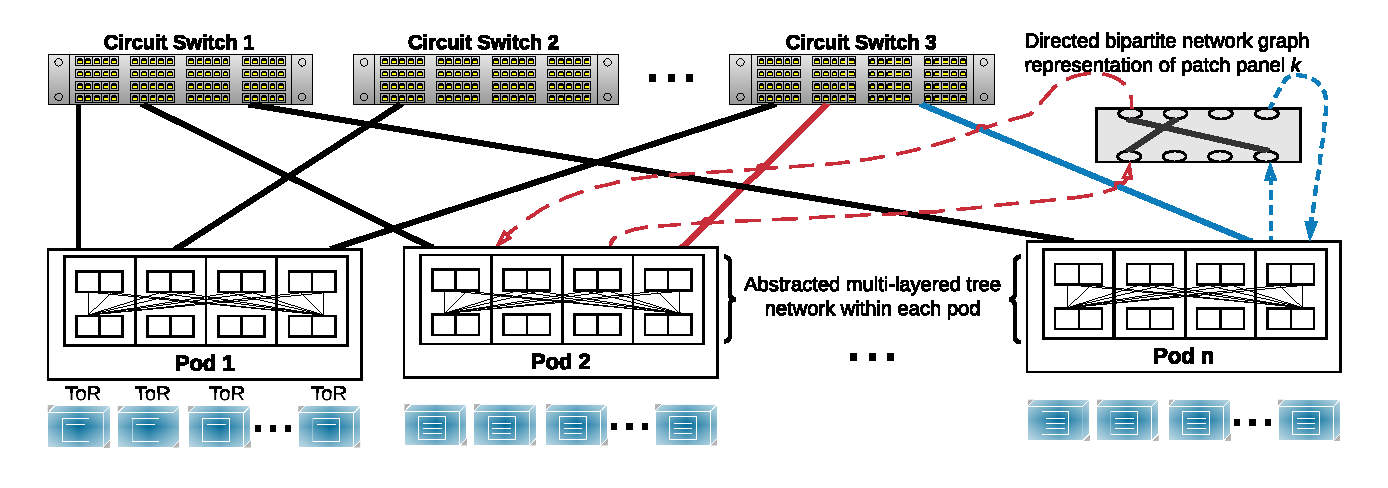
\includegraphics[draft=false, height= 1.6in,trim={0.7cm 0.6cm 0.7cm 0.7cm}, width=0.92\textwidth]{figures/helios_v2}
\caption{Helios topology fully interconnected via a patch-panel layer, alongside an illustration on the bipartite network graph representation of patch-panel $k$. All links in solid lines are bidirectional, and dotted links of the same color are the unidirectional representation of the same solid link.}
\label{direct_connect_topology}
\end{figure*}

\section{Introduction}

Based on established literature \cite{benson2010network, benson2009understanding}, we know that inter-rack traffic patterns tend to be highly skewed. This implies a high degree of traffic locality, and that all-to-all uniform traffic rarely occurs. In addition to traffic skewness, studies \cite{delimitrou2012echo} show that most data center fabrics demonstrate transient, bursty traffic behavior. These highly-skewed traffic naturally create network hotspots, and severely congesting network links while leaving other network links relatively underutilized. Furthermore, these transient bursts further complicates DCN design since predicting traffic patterns accurately is very difficult, if not close to impossible.

One way to ``even'' out highly-skewed traffic patterns is to load-balance using workload migration and clever job-placement \cite{jain2012topology}. However, as data center tends towards disaggregated hardware resources \cite{papaioannou2016benefits}, relying solely on intelligent workload placement will for link load-balancing will become increasingly difficult. This is because disaggregating compute resources from storage resources will force same workloads to be mapped onto dedicated clusters that are physically-separated. Even with perfect knowledge on job arrival and generated network traffic behavior, workload-placement alone cannot fundamentally even out the strong pairwise traffic pattern inherent to DC resource desegregation. \cite{reactor_liu2014}

To account for traffic skewness and variability, many reconfigurable data center topologies~\cite{farrington2011helios, cthrough_wang_2011, reactor_liu2014, hamedazimi2014firefly, ghobadi2016projector} have been proposed using different optical circuit switching technologies. Optical circuit switching incurs non-negligible reconfig time, which could significantly increase data center's control plan complexity. As a consequence, a lot of effort has been put into driving down the switching time of these switching technologies. An implicit assumption here is that fast switching is a ``must have'' in order for a control plane to react to rapid and bursty traffic changes. In this work, we would like to challenge this assumption, and answer the question, ``can slowly reconfigurable topology capture fast traffic dynamics?''

Another approach to even out out non-uniform traffic is through the use of congestion-aware routing algorithms. Most congestion-aware routing algorithms (i.e traffic engineering) balances link utilization across the network by deflecting traffic flow non-minimally to intermediate blocks first along less-congested paths. To first order, these congestion-aware routing schemes can introduce significant network delay to packets. More importantly, congestion-aware routing has the effect of creating network hotspots in other network areas, increasing overall traffic load within the network, and not to mention taking up precious bandwidth resources from other network resources. Therefore, it is clear that traffic engineering alone cannot sufficiently decongest and improve network throughput under many traffic permutations. 

In order to handle highly-skewed and vastly dynamic traffic behavior within DCNs, there has been much work dedicated to designing reconfigurable network topologies using dedicated switching hardware with very fast switching speeds. The key idea is to allow the topology to be reconfigured dynamically to the traffic changes. Some prominent examples that come to mind are the Firefly \cite{hamedazimi2014firefly} and ProjectTor \cite{ghobadi2016projector}, although many different topologies based on different hardware technologies have been proposed in established literature. The key concept that motivates these reconfigurable DCN topologies are more or less identical: to match the topology with the traffic matrix in either a predictive or reactive manner. A lot of effort has been put into driving down the switching time of these switching technologies in hopes of driving down the cost of topology reconfiguration. Unfortunately, to fully interconnect even a moderately-sized DCN network to full bandwidth capacity using these specialized switching hardware can be overly cost-prohibitive, therefore making them impractical for deployment until the underlying technology has matured.

That being said, we set out by asking the question: is it possible to design a static topology that is optimized not only for highly-skewed traffic, but also one that is robust under dynamic traffic changes? Answering this question requires us to first understand DCN traffic temporal behavior. Thus, we've conducted some preliminary studies using historical traffic data collected from our production data centers. Based on the findings, we observed that all DCN fabrics exhibit remarkable multi-modal traffic behavior in the time-domain, despite the fact traffic matrix show little to no temporal patterns. What this means is that there exists a small set of recurring traffic matrices that can be used to accurately represent all other traffic matrices, with only very few outliers. 

These findings lead us to believe that, perhaps counter-intuitively, by designing a static topology optimized for all of the traffic modes using only commercial patch panels can enhance network performance while still being sufficiently robust to dynamic traffic change. In other words, we believe that a sufficiently well-designed \textbf{static} topology can enhance network throughput under highly-skewed traffic patterns, while still being able to perform well under highly \textbf{dynamic traffic changes}.  

Therefore, our contributions in this work is fourfold:
\begin{itemize}
    \item We observed and surmise that DCN traffic can be represented using a small set of recurring traffic modes.
    \item We offer a traffic-aware topology design methodology on a DCN interconnected using off-the-shelve commodity patch panels to design a \textbf{static} topology that is highly robust to long term traffic change.
    \item We present a routing-topology co-optimization technique that considers multiple traffic modes which also accounts for DCN heterogeneity.
    \item We propose 2 highly scalable, polynomial-time, and mathematically-guided algorithms for mapping fractional target topology onto the physical patch-panel with close-to-optimal performance.
\end{itemize}

Based on our proposed methodology, we present simulation results using production traffic data on 4 DCN fabrics, with the topology computed at the start of the month and remains static throughout the entirety of the month. For baseline comparison, we use a uniform topology load-balance using just congestion-aware traffic engineering with global traffic knowledge. Our month-long timeseries evaluation shows that using our proposed methodology consistently outperforms a uniform topology in maximum link utilization by 8\% to 10\%. Similarly, our results show that the average packet hop count can be significantly improved, with more than 90\% of the traffic taking a direct-path towards its destination. These results suggest that subjected to the same traffic load, our proposed methodology can both decongest network links (by lowering max link utilization) while ensuring most traffics are able to stay within direct paths, thereby lowering average link congestion levels and average network-traversal latency. 

\begin{comment}
The rest of this paper is structured as follows: Section \ref{section_background} provides an overview of related works and background on reconfigurable DCN topologies. Section \ref{section_challenges_overall_approach} then addresses the various challenges encountered in our work, and describes the high-level ideas of our approach. Sections \ref{section_detecting_traffic_modes}, \ref{section_fractional_topology}, \ref{section_patch_panel_mapping} and \ref{section_reconfiguration_algo_analysis} details our traffic-aware topology engineering methodology and subsequently analyzes its runtime and optimality. Then, we evaluate the efficacy of topology engineering on actual production DCN fabrics using production traffic data through timeseries analysis. The penultimate Section \ref{section_when_to_reconfigure} briefly discusses the circumstances in which the topology reconfiguration should be triggered. Finally, we draw our conclusion and propose directions for future work in Section \ref{section_conclusion}.
\end{comment}
%% Maybe don't have to detail it so much in intro, just combine sections 5,6,7,8 into one for instance.

\begin{figure*}[ht!]
\centering
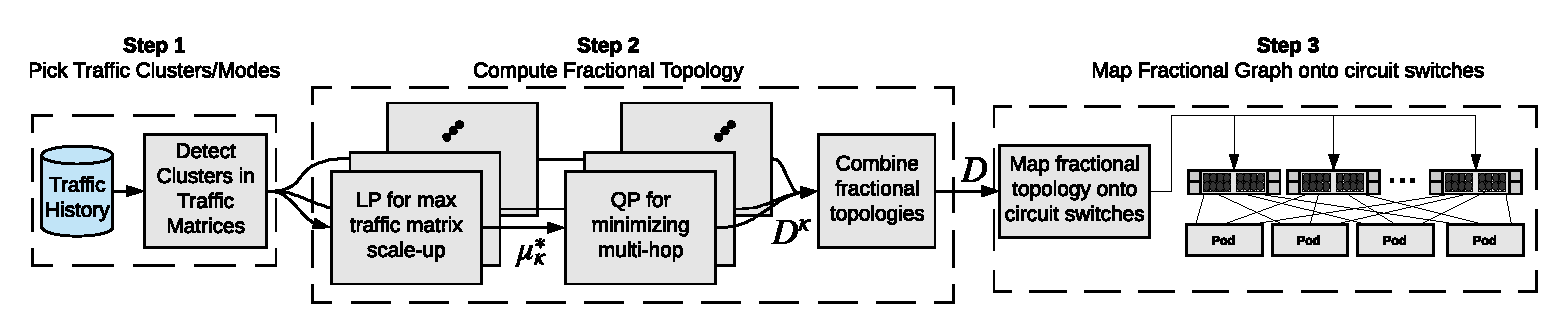
\includegraphics[trim={0.5cm 0.8cm 0.1cm 0.7cm}, width=\textwidth, scale=1.2]{figures/topology_engineering_overall_algorithm} 
\caption{Overall traffic-aware topology engineering work flow}
\label{topology_engineering_overall_workflow}
\end{figure*}
\section{Background \& Motivation}\label{section_background}

Over the course of the past decade, the increasing role of cloud computing has led to more emphasis on intelligent DCN design. As a result, the research community to study DCN topologies that are scalable, cost-effective and failure-tolerant using commodity static switches with much more rigor. Within the realm of established literature, the proposed topologies, and some defining examples, can be broadly listed as follows: 
\begin{itemize}
    \item \textbf{Clos topologies}: Fat-tree \cite{al2008scalable}, Google's Jupiter \cite{singh2015jupiter}, Microsoft's tapered fat-tree \cite{liu2013f10, greenberg2009vl2}
    \item \textbf{High-radix, low-diameter topologies}: Dragonfly \cite{kim2008dragonfly, teh2017design}, Slimfly \cite{besta2014slim}, HyperX \cite{ahn2009hyperx}
    \item \textbf{Direct connect topologies}: BCube \cite{guo2009bcube}, DCell \cite{guo2008dcell}, Dahu \cite{radhakrishnan2013dahu}
    \item \textbf{Random graph-based topologies}: Xpander \cite{valadarsky2015xpander}, S2 \cite{yu2016space}, Jellyfish \cite{singla2012jellyfish}
\end{itemize}

One major disadvantage these static topologies suffer from is that they are not designed with traffic patterns in mind, thus making them suboptimal to highly-skewed traffic patterns and dynamic traffic changes. In order to adapt to traffic dynamism, many reconfigurable topologies using sophisticated circuit-switches \cite{vahdat2011emerging, liu2010scaling, fields2010transceivers, zhou2017datacenter} have been proposed. The central idea to these topologies is to utilize sophisticated switching hardware to dynamically reconfigure the topology based on either predicted or measured traffic changes. Prominent examples include free-space optics(FSO)-based technology like ProjectToR \cite{ghobadi2016projector} and Firefly \cite{hamedazimi2014firefly}, and wireless beamforming-based in \cite{zhou2012mirror}. Several hybrid topologies \cite{farrington2011helios, cthrough_wang_2011, reactor_liu2014} have also been proposed by combining electrical packet switches and optical circuit switches within the DCN, and rely on complex scheduling techniques \cite{liu2015scheduling, porter2013integrating} to optimize for network throughput. Meanwhile, increasing maturity in MEMS technology has also led to the debut of RotorNet \cite{rotornet_mellette2017} and Proteus \cite{singla2010proteus}. Unfortunately, frequent topology reconfiguration topology introduces significant complexities within network control plane, including, but not limited to:
%% remove the details for what switching technologies are actually used by each of these topologies
\begin{enumerate}
    \item raising software complexity since the routing tables will be forced to re-computed upon topology change.
    \item incurring non-trivial connection down time during circuit reconfiguration, causing disruption to un-buffered traffic flow.
    \item rendering network performance highly susceptible to degradation due to innacurate traffic prediction.
\end{enumerate}

%% cite the traffic study papers as well
The aforementioned challenges can be avoided using a static topology, yet the common consensus is that static topologies do not possess sufficient flexibility to adapt to dynamic traffic changes. Conventional wisdom suggests that robustness to traffic dynamism and topology staticity are two topological properties that are fundamentally at odds. Our preliminary study on temporal traffic behavior using historical production traffic data, however, shows findings that seek to challenge this conventional wisdom. These findings are presented in Figure \ref{fig:cosine_sim} and elaborated in Section \ref{section_detecting_traffic_modes}. There, we will find that all DCN fabrics demonstrate $\kappa$-traffic modal behavior, even though predicting a traffic matrix at a given time accurately with high degrees of confidence is exceedingly difficult. In other words, all traffic matrices aside from a select few outliers can be represented by a small set of recurring traffic ``modes''. Based on these findings, we posit that a static topology optimized for all of the traffic modes can be robust under dynamic traffic change. 

Therefore, we depart significantly from established approaches to traffic-aware DCN topologies by proposing a (perhaps counter-intuitively) \textbf{static} topology engineering methodology which is capable of handling dynamic traffic changes, and fully implementable on commodity patch panel that are both cheap and easy to operate. By designing a topology that is static for prolonged periods of time (on the timescale of DC-expansions), we can also nullify the need for a complex control plane or building dedicated hardware that is otherwise required in other reconfigurable topologies, thereby reducing potential control-plane failures, operational and construction cost. 

The topology we are considering in this paper is heavily-inspired by Helios \cite{farrington2011helios}, with the core switches replaced entirely with patch panels. The merits of utilizing a patch panel reconfigurable layer is discussed in detail in Zhao et al. \cite{zhao2018minimal}. Figure \ref{direct_connect_topology} provides an illustration of the topology. We treat the network as a directed network, hence each link can only carry traffic in one direction. Ingress and egress ports are dedicated to receiving and sending traffics, respectively. Each bidirectional link is formed by combining two directed links in opposite directions. We also assume patch panel-asymmetry, meaning that A's egress port being connected to B's ingress port does not imply that A's ingress port is connected to B's egress port.

\section{Challenges \& Overall Approach}\label{section_challenges_overall_approach}
%% A lot of the complexities of reconfigurable topology problem spawns from algorithmic and mathematical reasons. 

The first of the biggest challenges we face in the context of this work is to figure out how to deal with transient traffic changes using a static topology. This restriction is imposed due to the fact that building a data center of our scale that is fully-interconnected at full-capacity using dedicated switching hardware is cost-prohibitive. Having established that DCN fabrics exhibit multi-modal (henceforth denoted as $\kappa$-modal) traffic behavior in Section \ref{section_background}, we posit that designing a topology optimized for all traffic modes can render a static network robust to traffic changes. To identify these traffic modes, we treat all historical traffic matrices as points in high-dimensional space, as shown in Step 1 of Figure \ref{topology_engineering_overall_workflow}. This essentially reduces the problem problem of finding traffic modes to that of locating traffic clusters in high-dimensional space, a common machine learning problem which can be done efficiently using various available clustering algorithms. Although counter-intuitive, our simulation results done using production DCN traffic in Section \ref{section_timeseries_analysis} show that this idea works very well in-practise.

The next major challenge lies in computing an optimal logical topology for a given set of traffic demands. Unlike our previous challenge which stems from hardware restrictions and impracticalities of frequent reconfiguration using patch panels, this challenge is mathematical in nature and is a problem universal to all reconfigurable topologies. The main source of complexity is due to two reasons: 1) the logical topology needs to be in integer form, and 2) when the network is not fully-connected (i.e not all combinations of port connections are possible due to them being physically-wired to different patch panels). These reasons make the problem a strongly NP-hard combinatorial problem, as shown in Foerster et al.\cite{foerster2018characterizing}. In this work, we take a routing-topology co-optimization approach. By considering both routing and topology within the same topology engineering problem, we can effectively optimize for a given network performance metric (such as link congestion, packet hop-count, etc) directly, ensuring that the computed logical topology is indeed optimized under a given traffic load when measured. However, computing the logical topology directly by formulating an integer linear program (ILP) is too computationally-expensive. So, we approach this problem is 2 steps, which form Step 2 and 3 of Figure \ref{topology_engineering_overall_workflow}.

In Step 2, we first co-optimize a topology alongside routing by assuming a fully-connected network where all port pairs can be interconnected with fractional link counts. This can allows to formulate step 2 as a simple linear program (LP) that can be solved quickly. Finally, we attempt to map the fractional optimal topology onto the patch panel layer with the objective of matching the logical topology to the fractional topology. Note this this portion is where the NP-hardness of the problem comes from, therefore we cannot guarantee optimality of solution.

\begin{comment}
Step 2 has two sources of complexity: 1) we want to co-optimize routing and topology, and 2) the logical topology needs to be in integer form. 


The main question we want to answer is this: given a pool of traffic data, and a physical network topology, how do we determine the best logical topology to deploy for enhanced network performance? It is well-know that traffic-aware topology engineering presents a difficult combinatorics challenge. This problem is further compounded by limitations on reconfiguration frequency imposed by the deployment of commodity patch-panels which require manual-rewiring in our DCN fabrics. As such, whatever topology engineering methodology we propose must result in long-term (month-long timescales) performance enhancements under different and changing traffic patterns in order to be feasible. But how can we employ topology engineering when traffic can be unpredictable, especially on such significant monthly timescales? Fortunately, while it is incredibly difficult (if not outright impossible) to predict the traffic matrix at time $t$ based on historical traffic behavior with any certainty, it is highly likely that the traffic matrix will look like one of the few traffic ``modes``, as stated in our findings in Section \ref{section_background}. Given this finding, we now need to answer two main questions:

\begin{itemize}
    \item How do we detect these traffic modes?
    \item How do we compute a logical topology that is optimal for all these traffic modes?
\end{itemize}

To answer the first question, we treat traffic matrices as high-dimensional vectors and locate the modes using clustering algorithms. This allows us to find the traffic modes by locating the distinct clusters of traffic matrices. In this work, we've employed a simple $k$-means-clustering technique to , though may different clustering techniques like expectation maximization (EM) clustering may also be employed. This implies that clusters are located based on how close they are in terms of euclidean distance. Although it is an intuitive measure, it may not necessarily yield the best quality of traffic modes. A detailed discussion of the relative merits of different clustering method and metrics is out of the scope of this work, and we would like to give these questions rigorous treatment in future works.

The second question is difficult due to two key properties: 1) the final solution (i.e logical topology) has to be in integer form, and 2) the problem can be mapped onto a three-dimensional matching problem\cite{irving1994three}, which is proven to be NP-hard. We tackle this problem using a two-stage process. Firstly, a fractional topology optimize for all $k$ traffic modes is computed assuming a fully-connected network. This assumption is used to prevent the linear program (LP) formulated from suffering scalability issues as the variable space expands from $O(n^2)$ to $O(kn^2)$ upon considering patch-panel layer, where $n$ and $k$ denote the number of pods and number of patch-panels, respectively. By assuming a fully-connected network, then, we can easily formulate this problem as smaller LP that is easily solvable. Here, we employ a routing-topology co-optimization strategy in which the fractional topology solution is computed while considering routing flow weights. Combining routing and topology computation is crucial, as this allows us to optimize for the measured network metric (link congestion, packet latency, etc) of interest directly, since network metrics are a measured effect of both topology and routing under a given traffic load.

With the fractional topology computed, we attempt to faithfully map it onto the patch-panels such as the final logical topology best matches this fractional target topology. Note that this challenge is universal to all reconfigurable topology problems under a none-fully connected network assumption, regardless of the frequency of reconfiguration. We believe that our solution can be equally applied to other reconfigurable topology equipped with optical switches for high-frequency topology-reconfiguration. The overall work flow of our approach, from detecting traffic modes to obtaining a logical topology, is illustrated in Figure \ref{topology_engineering_overall_workflow}.
\end{comment}



%% This is the main discussion section for the algorithm
\section{Definitions \& Notations}\label{section_notations}
\subsection{Definitions}
We briefly define several recurring terminologies in the context of this work:
\begin{itemize}
\vspace{-4pt}
    \item \textbf{Physical Topology} Describes the physical connectivity between the pods and the patch panels, represented as a directed graph.
    \item \textbf{Logical Topology} Describes the connectivity (i.e number of integer links) between pods, abstracting away the layer of patch-panels.
    \item \textbf{Fractional Topology} Logical topology assuming that inter-pod link counts can occupy non-integer values. 
\end{itemize}

\subsection{Notations}
%% include the table of notations here
\begin{table}
\begin{tabular}{|p{2.7cm}|p{5.3cm}|}
\hline
$S = \{s_1, ..., s_n\}$ & Set of all $n$ pods\\
\hline
$O = \{o_1, ..., o_k\}$ & Set of all $k$ patch-panels\\
\hline
$x_{ij}^k$ & Number of pod $i$'s egress links connected to pod $j$'s ingress links through $o_k$\\ 
\hline
$\Psi(\mathbf{x})$ & Quality function of patch-panel configuration\\
\hline
$T = [t_{ij}] \in \mathbb{R}^{n\times n}$ & Traffic matrix, where $t_ij$ denotes the sent from $s_i$ to $s_j$\\ 
\hline
$D = [d_{ij}] \in \mathbb{R}^{n\times n}$ & Fractional topology, where $d_ij$ denotes the number of $s_i$ egress links connected to ingress links of $s_j$\\ 
\hline
$h_{eg}^k(s_i), h_{ig}^k(s_j)$ & Number of physical egress links connecting $s_i$ to $o_k$, and number of physical ingress links of $s_j$ to $o_k$, respectively\\
\hline
$r_{eg}^i, r_{ig}^i$ & Number of egress and ingress links, respectively, owned by $s_i$\\
\hline
$b_i$ & Link bandwidth of $s_i$\\
\hline
$P_{ij}$ & Set of all viable routing paths from $s_i$ to $s_j$ within the topology\\
\hline
$P(e_{ij})$ & Set of all paths that traverses logical links connecting $s_i$ to $s_j$\\
\hline
$l_p$ & Length/hop count of path $p$ \\
\hline

$\omega_{p}$ & WCMP weight allocated along path $p$ \\
\hline
\end{tabular}
\caption{Commonly-used notations} 
\label{table:notations}
\end{table}
 Before giving a rigorous treatment to the topology engineering problem, we dedicate this section to introducing a series of recurring notations that will be used throughout this paper. These notations are tabulated in Table \ref{table:notations}. For the sake of convenience, we shall abuse the notation $\mathbf{x} \in \mathbb{R}^{\lVert S \lVert \times \lVert S \lVert \times \lVert O \lVert}$ to denote the vector of $x_{ij}^k \; \forall \; i, j \in S, k \in O$, and $\mathbf{x}^k \in \mathbb{R}^{\lVert S \lVert \times \lVert S \lVert}$ to denote the vector of $x_{ij}^k \; \forall \; i, j \in S$ associated with a particular $k$. Similarly, we shall abuse the vector notation $\mathbf{d} = \{d_{ij} \; | \; i, j \in S\}$, and $\boldsymbol{\omega_p} = \{w_p \; | \; p \in \bigcup\limits_{i, j \in S}P_{ij}\}$.

As shown in Figure \ref{direct_connect_topology}, we assume each patch panel can be represented as a bipartite network flow graph. In our asymmetric topology model, $x_{ij}^k \neq x_{ji}^k$ for any $i \neq j$ in general. 


%\section{Traffic-aware Topology Design Benefits}\label{section_topology_engineering_benefits}
%\input{./sections/reconfiguration_methodology/toy_example.tex}

\section{Step 1: Detecting Traffic Modes} \label{section_detecting_traffic_modes}
%% 1) show that k means clustering and pick the ideal k value, show diminishing return of increasing k, and show that only k = 2 or k = 3
Due to the switching speed of our direct-connect topology being limited by the patch-panel layer, choosing the right traffic matrix for a monthly redesign of the logical topology is extremely crucial. Based on our observations, the volume of traffic changes very frequently, but the traffic pattern doesn't change all that much for prolonged periods of time, with sporadic changes in pattern. Therefore, we do not need to reconfigure the topology so frequently since the traffic patterns do not change regularly. But over-fitting the topology to serve the long term traffic pattern might lead to significant performance degradation and congestion for the occasional drastic changes. A robust topology should be capable of serving multiple traffic patterns well. Therefore, the problem statement becomes: Given a set of traffic matrices that has been measured, we would like to pick a set of representative traffic matrices.  \cite{zhang2005finding}. To reiterate, given a set of input traffic matrices, $T = \{T^1, T^2, ..., T^m\}$, identify a set of traffic matrices $Y = \{Y^1, Y^2, ..., Y^l\}$ that are ``representative'' of $T$ such that $l \leq m$. Mathematically, we want to pick a set of $\kappa$ matrices that is closest to all the points in $T$. 

This problem is similar to that in \cite{zhang2005finding}. Unlike the \textit{CritMat}, however, we do not need to take the a set of traffic matrices that also dominates the others, since we only care about the pattern and not the sheer magnitude of the traffic matrices. In other words, we only care about normalized traffic matrices. To find the representative matrices, we employ $\kappa$-means-clustering technique to select $\kappa$ representative traffic matrices. While a higher $\kappa$ gives us more clusters, it becomes progressively harder to design a topology that can serve high $\kappa$ values, since vastly different traffic modes may introduce many mutually-conflicting constraints. Also, as $\kappa$ increases, there superposition of all modes may tend towards a uniform traffic matrix, hence rendering topology engineering completely unnecessary. It turns out that selecting $\kappa = 2, 3$ tends to be good enough choices.\\
\begin{comment}
\begin{figure}[t!]
    \centering
    \includegraphics[width=\linewidth,scale=0.8]{./figures/diminishing_returns.pdf}
    \caption{Diminishing returns of increasing $k$}
    \label{diminishing_returns}
\end{figure}
\end{comment}

%% include the figure for diminishing return of k here.
\begin{figure}[t]
    \centering
    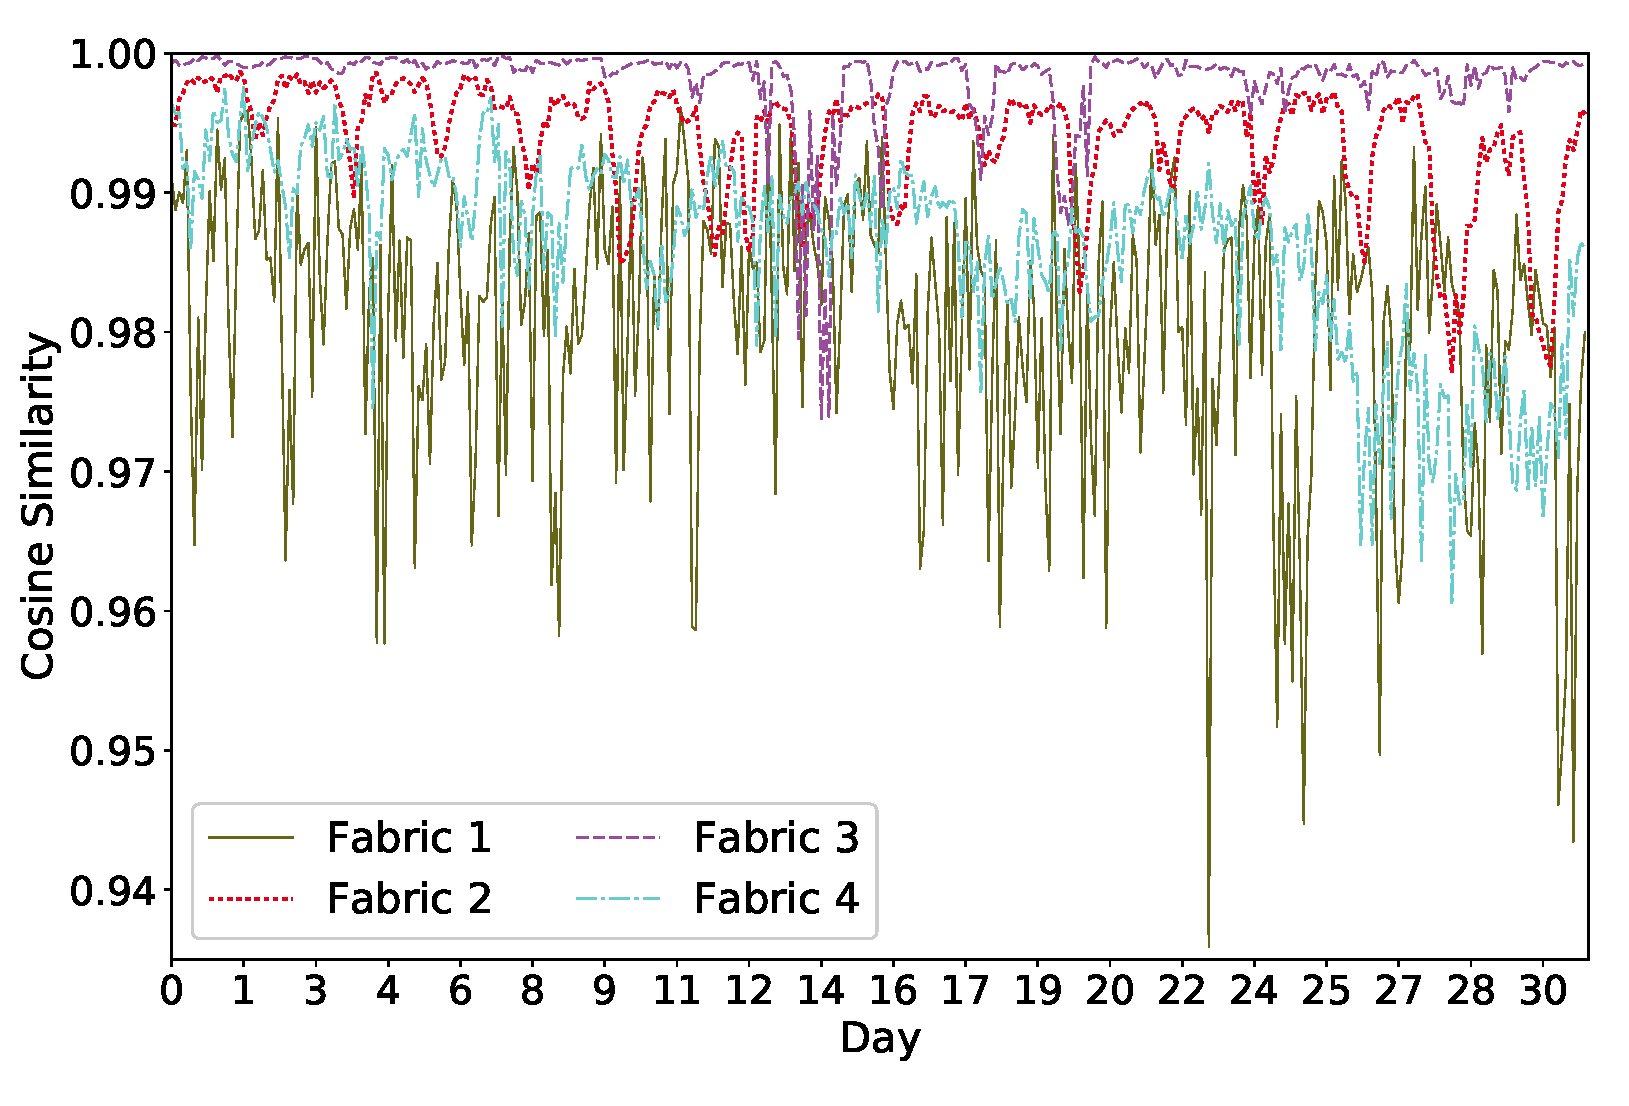
\includegraphics[width=3.3in,height=2.25in,trim={0.7cm 1.2cm 0.4cm 0.7cm}]{./figures/cosine_sim.eps}
    \caption{Cosine similarity between hourly traffic matrix using previous month's traffic modes}
    \label{fig:cosine_sim}
\end{figure}

%%%%%%%%%%%%%%%%%%%%%%%%%%%%%%%%%%%%%%%%%%%%%%%%%%%%%%%%%%%%%%%%%%%%%%%%%%%%%%%%%%%%%
%%%%%%%%%%%%%%%%%%%% Deriving Optimal Fractional Graphs%%%%%%%%%%%%%%%%%%%%%%%%%%%%%%
%%%%%%%%%%%%%%%%%%%%%%%%%%%%%%%%%%%%%%%%%%%%%%%%%%%%%%%%%%%%%%%%%%%%%%%%%%%%%%%%%%%%%
\section{Step 2: Computing Fractional Topology}\label{section_fractional_topology}
At this point, we've obtained $\kappa$ representative traffic matrices, each representing a recurring traffic mode. Using these traffic modes, we detail a topology-routing co-optimization methodology to compute an optimal fractional topology. In this step, our goal is to compute a fractional topology that is optimized for all of the traffic modes found, as discussed in Section \ref{section_detecting_traffic_modes}. The logic employed here is that a fractional topology that is optimized for all of the traffic modes will allow our topology to cover sufficient grounds to account for traffic changes over time. 

\subsection{Definitions}
We start off by giving a more rigorous definition of what a fractional topology is. As its namesake suggests, the number of links between two pods. In addition to non-integer inter-pod link counts, a fractional topology must satisfy additional constraints, as given by:

%% Definition 1
\begin{definition}
$D = [d_{ij}] \in \mathbb{R}^{n \times n}$ is a fractional topology i.f.f it satisfies 
\begin{equation}
\sum\limits_{j \in S} d_{ij} \leq r_{eg}^i \; \forall \; i \in S 
\label{constraint:egress}
\end{equation}
\begin{equation}
\sum\limits_{i \in S} d_{ij} \leq r_{ig}^{ j} \; \forall \; j \in S
\label{constraint:ingress}
\end{equation}
\label{defn:fractional_graph}
\end{definition}
Note that (\ref{constraint:egress}) and (\ref{constraint:ingress}) denote the egress degree constraints and ingress degree constraints, respectively. These are the most fundamental set of constraints that satisfy the out-degree and in-degree of each pod. In addition, there are two main properties of the fractional topology we wish to discuss. Firstly, the fractional topology noticeably ignores the patch panel layer. This is done because the accouting for the patch panel layer carries neither mathematical nor algorithmic significance. Not only does its accounting unnecessarily increases the number of variables needed to represent a fractional topology, the fact that the panel layer will be considered in Step 3 of Figure \ref{topology_engineering_overall_workflow} as we map the fractional topology into an integer logical topology renders it redundant. Secondly, fractional number of links interconnect two pods are allowed because it permits us to compute a fractional topology by formulating a LP instead of an ILP, which has significantly higher complexity.

Next, we define $\Omega(T, D) = \{\omega_p \; | \; p \in \bigcup\limits_{(i, j) \in S \times S}P_{ij}\}$ as the multi-hop routing solution of traffic matrix $T$ on fractional topology $D$. For any pair of traffic matrix and fractional topology,  we define the meaning for feasibility of $(T , D)$ as:

%% Definition 2
\begin{definition}
$(T, D)$ is feasible i.f.f there exists a routing solution $\Omega(T, D)$ s. t:
\begin{equation}
    t_{ij} = \sum\limits_{p \in P_{ij}}\omega_p \quad \forall \; i, j \in S
\label{constraint:meet_demands}
\end{equation}
\begin{equation}
    \sum\limits_{p \in P(e_{ij})} \omega_{p} \leq d_{ij}b_{ij} \quad \forall \; i, j \in S
\label{constraint:bandwidth_exceed}
\end{equation}
\label{defn:feasible_fractional_graph}
\end{definition}
Constraint (\ref{constraint:meet_demands}) enforces $(i, j)$ traffic demands to be satisfied via all routable paths, while constraint (\ref{constraint:bandwidth_exceed}) ensures that the traffic flowing through each link cannot exceed its bandwidth. Simply put, $(T, D)$ is feasible if there exists a routing solution for $T$ on $D$ such that all traffic flow demands can be met without exceeding $D$'s inter-pod link bandwidths. 

%% Subsection 2
\subsection{Finding the Best-fitting Fractional Topology}
For any given traffic mode matrix, $T_\kappa$, we want to find the corresponding fractional topology of best fit, namely $D_\kappa^*$. For $T_\kappa$, the fractional topology that has the best-fit is defined as:
\begin{enumerate}
    \item[1.] $D_\kappa^*$ should maximize $\mu_\kappa$ for all feasible $(\mu_\kappa T_\kappa, D_\kappa)$.
    \item[2.] $D_\kappa^*$ should be most similar to $T_\kappa$
\end{enumerate}
Fulfilling the first property makes a fractional topology merely a ``good'' fractional topology. There may be many such fractional topologies that can maximize $\mu_\kappa$, since fundamentally property 1 only optimizes for the hottest pod, and does not place much emphasis on the other pods that do not eject or inject as much traffic into the network. Therefore, we strengthen the best-fit definition by introducing property 2, which essentially selects the fractional topology that looks most similar to $T_\kappa$ among the set of fractional topologies that maximizes $\mu_\kappa$. Assuming that $\mu_\kappa^*$ denotes the maximum scale-up factor among the set of all feasible $(\mu_\kappa T_\kappa, D_\kappa)$, we find the best fitting fractional topology, $D$, for each traffic mode using:
\begin{equation}
\begin{aligned}
\min\limits_{\boldsymbol{\omega_p}, \mathbf{d}} \;& \quad \sum_{i, j \in S} \; \sum_{p \in P_{ij}(l_p > 1)}\big(\omega_{p}\big)^2 \\
\text{s. t: } & 1) \; \sum_{p \in P_{ij}} \omega_{p} = \mu_{\kappa}^* t_{ij}, \quad \forall \; i, j \in S \\
& 2) \sum\limits_{p \in P(e_{ij})} \omega_{p} \geq \mu_{\kappa}^* \; d_{ij} b_{ij}, \quad \forall \; i, j \in S\\
& 3) \quad (\ref{constraint:egress}) \; , \; (\ref{constraint:ingress})
\end{aligned}\label{fractional_graph_qp}
\end{equation}

At this point, we've obtained the best-fitting fractional topology to each of the traffic modes. We need to combine all these individual fractional topologies into one fractional topology with which we will map onto the patch panels to obtained the final integer logical topology. For computing the combined fractional topology, we linearly combine the individual best-fitting fractional topologies by formulating the following LP:
\begin{equation}
\begin{aligned}
 & \max\limits_{\alpha > 0, \mathbf{d}^*} \; \quad \alpha \\
 \text{s. t: } & 1) \quad d_{ij}^* \geq \; \alpha \; d_{ij}^\zeta, \; \forall \; i, j \in S, \; \zeta \in \{1, 2, ..., \kappa\} \\
  & 2) \quad [d_{ij}^*] \text{ is feasible}
\end{aligned}\label{combine_fractional_graphs}
\end{equation}
Where $\alpha$ is the scaling factor of each individual fractional graph. Constraint 1 in (\ref{combine_fractional_graphs}) is imposed so that each $(i, j)$ fractional link in the combined fractional graph, $d_{ij}^*$, can dominate all other $\alpha$-scaled $d_{ij}^\zeta \; \forall \; \zeta \in \{1,2, ..., \kappa\}$.













\begin{comment}
In this section, we detail a routing-topology co-optimization methodology used for computing an optimal fractional topology given a set of traffic matrices. As mentioned briefly in Section \ref{section_challenges_overall_approach}, we've decided to tackle the optimal logical topology computation by splitting the large problem into two smaller, more easily-solvable problems. In computing the optimal topology, we've decided to ignore the patch panel layer and assume full-connectivity, which is motivated by two reasons: Firstly, considering the patch-panel layer increases the number of variables and constraints required to formulate the LP, which incurs scalability issues when optimizing for larger topologies. Secondly, including the patch-panel layer (which will be considered in Step 3 regardless) brings about negligible improvement (if any) to the optimality of our final integer logical topology. 

Step 2 of Figure \ref{topology_engineering_overall_workflow} shows that instead of considering all traffic modes in the same fractional derivation computing, we compute a fractional topology optimal for each traffic mode, and then finally combine all these topologies using LP. This is because formulating an LP that considers all the traffic modes together greatly increases the complexity of the problem. Based on our experience, solutions obtained from LP's tend to be unstable, therefore we employ a quadratic program (QP) to stabilize the fractional topology for each traffic mode. Finally, all the $\kappa$ fractional topologies are linearly combined using LP.

Given that we assume full-connectivity here, the only physical constraints to be imposed for computing fractional topologies are:
\begin{equation}
\sum\limits_{j \in S} d_{ij} \leq r_{eg}^i \; \forall \; i \in S 
\label{constraint:egress}
\end{equation}
\begin{equation}
\sum\limits_{i \in S} d_{ij} \leq r_{ig}^{ j} \; \forall \; j \in S
\label{constraint:ingress}
\end{equation}
Constraints (\ref{constraint:egress}) and (\ref{constraint:ingress}) upper-bounds the number of links formed by $s_i$ with its peer pods to its total number of egress links and ingress links, respectively. Now, given a traffic mode $T^\kappa$, we want to obtain an fractional topology that can support the largest scale-up of $T^\kappa$ under multihop routing, which can be formulated as the following LP:

\begin{equation}
\begin{aligned}
 & \max\limits_{\mu_\kappa, \boldsymbol{\omega_p}, \mathbf{d}} \; \quad \mu_{\kappa} \\
\text{s. t: } & 1) \; \sum_{p \in P_{ij}} \omega_{p} = \mu_{\kappa} \; t_{ij}^k, \quad \forall \; i, j \in S \\
& 2) \sum_{p \in P(e_{ij})} \omega_{p} \leq d_{ij} b_{ij}, \; \forall \; i, j \in S\\
& 3) \quad (\ref{constraint:egress})\; , \; (\ref{constraint:ingress})
\end{aligned}\label{fractional_graph_lp}
\end{equation}
Where $b_{ij} = \min(b_i, b_j)$ and $\mu_{\kappa}$ is the traffic matrix scale-up factor for traffic mode $\kappa$. Constraint 1 enforces all scaled-up $i$ to $j$ traffic demands to be satisfied via all routable paths, while constraint 4 ensures that the traffic flowing through each link cannot exceed its bandwidth. Unfortunately, the linear nature of (\ref{fractional_graph_lp})'s objective function causes the solution to suffer from stability issues. (\ref{fractional_graph_lp}) implies that there may be many different fractional topologies that can support the same scale-up factor, $u^\kappa$, with some viable fractional topologies perhaps relying more heavily on multi-hop routing rather than direct-hop routing. We know that relying on multi-hop routing not just increases the delay of each packet, but could also inadvertently congest other network links as overall traffic increases. To solve this issue, we extract the each traffic mode's maximal scale-up factor, $\mu_\kappa^{*}$, by solving (\ref{fractional_graph_lp}). Using the computed scale-up factor, we stabilize the fractional topology solution using a the strongly-convex properties of a quadratic program (QP) with linear constraints that acts as a solution ``filter''. So, for each traffic mode, the objective of this quadratic program is set to minimize multi-hop routing as much as possible while still supporting the same scale-up factor:
\begin{equation}
\begin{aligned}
\min\limits_{\boldsymbol{\omega_p}, \mathbf{d}} \;& \quad \sum_{i, j \in S} \; \sum_{p \in P_{ij}(l_p > 1)}\big(\omega_{p}\big)^2 \\
\text{s. t: } & 1) \; \sum_{p \in P_{ij}} \omega_{p} = \mu_{\kappa}^* t_{ij}, \quad \forall \; i, j \in S \\
& 2) \sum\limits_{p \in P(e_{ij})} \omega_{p} \geq \mu_{\kappa}^* \; d_{ij} b_{ij}, \quad \forall \; i, j \in S\\
& 3) \quad (\ref{constraint:egress}) \; , \; (\ref{constraint:ingress})
\end{aligned}\label{fractional_graph_qp}
\end{equation}
Where $P_{ij}(l_p > 1) = \{p \; | \; p \in P_{ij} \cap l_p > 1\}$ denotes the set of routing paths from $s_i$ to $s_j$ with hop-counts greater than 1. To solve (\ref{fractional_graph_qp}), we use the OSQP library \cite{osqp}. By attempting to minimize multihop routing, (\ref{fractional_graph_qp}) indirectly forces the fractional topology to ``match'' the traffic matrix. This has the added benefit of making the $\kappa$-th traffic mode's fractional topology to remain fairly optimal for traffic matrices that fall within mode $\kappa$'s cluster.

With each traffic mode, $T^\kappa$'s stable fractional topologies computed, we combine them into one fractional topology using linear combination of the form:
\begin{equation}
\begin{aligned}
 & \max\limits_{\alpha, \mathbf{d}^*} \; \quad \alpha \\
 \text{s. t: } & 1) \quad d_{ij}^* \geq \; \alpha \; d_{ij}^\zeta, \; \forall \; i, j \in S, \; \zeta \in \{1, 2, ..., \kappa\} \\
  & 2) \quad (\ref{constraint:egress}) \;, \; (\ref{constraint:ingress})
\end{aligned}\label{combine_fractional_graphs}
\end{equation}
Where $\alpha$ is the scaling factor of each individual fractional graph. Constraint 1 in (\ref{combine_fractional_graphs}) is imposed so that each $(i, j)$ fractional link in the combined fractional graph, $d_{ij}^*$, can dominate all other $\alpha$-scaled $d_{ij}^\zeta \; \forall \; \zeta \in \{1,2, ..., \kappa\}$.
\end{comment}

%%%%%%%%%%%%%%%%%%%%%%%%%%%%%%%%%%%%%%%%%%%%%%%%%%%%%%%%%%%%%%%%%%%%%%%%%%%%%%%%%%%%%
%%%%%%%%%%%%%%%%% Mapping fractional graphs to patch-panel%%%%%%%%%%%%%%%%%%%%%%%%%%%
%%%%%%%%%%%%%%%%%%%%%%%%%%%%%%%%%%%%%%%%%%%%%%%%%%%%%%%%%%%%%%%%%%%%%%%%%%%%%%%%%%%%%

%% Lagrangian Duality
\section{Step 3: Mapping Fractional Topology onto Patch-Panels}\label{section_patch_panel_mapping}
Having computed the optimal fractional topology, $D^*$, previously, we now attempt to map $D^*$ onto the patch panels such that the final logical topology best matches the fractional topology. Unfortunately, we cannot ignore the patch panel layer here. Since the logical topology has to be in integer form, obtaining the perfect match to this problem is equivalent to an NP-hard three-dimensional matching problem \cite{irving1994three, foerster2018characterizing}. In this work, we present two different relaxation approaches inspired by techniques commonly employed in convex optimization that provide close to optimal solutions. Before diving into the details of each approach, we briefly discuss some common structures to the patch-panel problem:
\textbf{\\Hard / Physical Constraints: } This constraint states that the total number of integral flows that reach $s_j$ through $o_k$ cannot exceed the total physical links connecting the ingress ports of $s_j$ from $o_k$:
\begin{equation}\label{phy_constraint1}
    \sum_{i \in S} x_{ij}^k \leq h_{ig}^k(j) \quad \forall \; k \in O, \; j \in S
\end{equation}
By reciprocity, total number of integral flows through $o_k$ originating from $s_i$ cannot exceed the total number of physical links connecting the egress links of $s_i$ to $o_k$ .
\begin{equation}\label{phy_constraint2}
    \sum_{j \in S} x_{ij}^k \leq h_{eg}^k(i) \quad \forall \; k \in O, \; i \in S
\end{equation}
\textbf{Soft / Matching Constraints: } We also want to match the logical topology with the fractional topology, therefore the following constraints are introduced:
\begin{equation}\label{con_constraint}
    c_{ij}^- \leq \sum_{k \in O} x_{ij}^k \leq c_{ij}^+, \quad \forall \; i,j \in S
\end{equation}
Where $c_{ij}^- = \floor{d_{ij}}$ and $c_{ij}^+ = \ceil{d_{ij}}$. A logical topology is deemed to perfectly match the fractional topology if for every $(s_i, s_j)$ pod pair, the inequality in (\ref{con_constraint}) is satisfied. It is possible that certain permutations of $D$ do not have a feasible solution.In those cases, we simply aim to minimize the number of soft constraints violated.\\



\subsection{Lagrangian Dual Method}\label{section_lagrangian_dual}
We draw significant inspiration from Low et al. \cite{low1999optimization} in our approach with the Lagrangian dual method.
The act of transforming the primal problem into its Lagrangian dual problem introduces the dual variables that will be used to ``score'' the cost of forming each logical link. 
The dual problem is:
\begin{equation}
\begin{aligned}
\min\limits_{\mathbf{p}^\pm}\max\limits_{\mathbf{x}}\Bigg\{U(\mathbf{x}) & + \sum\limits_{i, j \in S} \bigg[p_{ij}^- \big( \sum\limits_{k \in O}x_{ij}^k - c_{ij}^-\big) -p_{ij}^+ \big( \sum\limits_{k \in O}x_{ij}^k - c_{ij}^+ \big) \bigg] \Bigg\} \\
\text{s.t } & 1) \quad (\ref{phy_constraint1}) \text{ and } (\ref{phy_constraint2})\\
\text{} & 2) \quad \mathbf{p^\pm}  \succcurlyeq 0
\end{aligned}
\label{eqn:langrangian_duality}
\end{equation}
Where $p^\pm$ are the dual variables, and $U(\mathbf{x})$ denotes the objective function of the primal problem. In our implementation, we chose the primal objective function to be:
\begin{equation} 
\begin{aligned}
U(\mathbf{x}) = \sum\limits_{i, j \in S} \sum\limits_{k \in O} -\big( x_{ij}^k - h_{ij}^k\big)^2
\end{aligned}
\label{eqn:lagrangian_primal_objective}
\end{equation}
Where $h_{ij}^k = \min\big(h_{eg}^k(s_i), h_{ig}^k(s_j)\big)$. We take advantage of the fact that $x_{ij}^k \leq h_{ij}^k \; \forall i, j \in S, \; k \in O$ to ``coerce'' the resulting logical topology to form more logical links through higher $x_{ij}^k$ values. This will force the logical topology solution to more fully-utilize the physical links available to them due to $U(\mathbf{x})$ behaving like a least-squared curve-fitting problem. In addition, a quadratic objective function possesses a strong convexity which stabilizes solution convergence. 

Observing (\ref{eqn:langrangian_duality}) closely gives us a good intuition on how this method works. The dual variables $\mathbf{p}^\pm$ essentially ``scores'' the cost of forming logical links between pods. For instance, when a particular pod pair $(s_i, s_j)$ is significantly under-provisioned (i.e $\sum\limits_{k \in O} x_{ij}^k < c_{ij}^-$), $p_{ij}^-$ will increase while $p_{ij}^+$ will decrease such that future patch panels will attempt to form more logical links between $(s_i, s_j)$. The opposite is true for when $(s_i, s_j)$ pair is significantly over-provisioned. In a sense, the regulatory behavior $\mathbf{p}^\pm$ exhibits a negative-feedback behavior by incentivizing or disincentivizing the formation of $(s_i, s_j)$ logical links at each patch panel until the soft constraint is met. Rearranging (\ref{eqn:langrangian_duality}) gives us: 
\begin{equation}
\begin{aligned}
\min\limits_{\mathbf{p}^\pm} \Bigg\{\Big[- \sum\limits_{k \in O} \min\limits_{\mathbf{x}^k} Q_k(\mathbf{x}^k)\Big] + \sum\limits_{i, j \in S}p_{ij}^+ c_{ij}^+ - \sum\limits_{i, j \in S}p_{ij}^- c_{ij}^- \Bigg\}
\end{aligned}
\label{eqn:lagrangian_duality_mcf}
\end{equation}
Where $Q_k(\mathbf{x}^k) \approx \sum\limits_{i, j \in S}\big[p_{ij}^+ - p_{ij}^- - 2 h_{ij}^k + 2 x_{ij}^k{}^*\big]x_{ij}^k$. Note that $\min\limits_{\mathbf{x}^k}Q_k$ is simply a Min-cost Flow (MCF) problem for $o_k$ with $x_{ij}^k$ being the arc flow and $[p_{ij}^+ - p_{ij}^- - 2 h_{ij}^k + 2 x_{ij}^k{}^*]$ the cost per unit flow, which is obtained by applying first order linear approximation on an otherwise quadratic $Q_k(\mathbf{x}^k)$ evaluated at $x_{ij}^k = x_{ij}^k{}^*$. Interestingly, (\ref{eqn:lagrangian_duality_mcf}) decouples an otherwise difficult-to-solve convex optimization problem with integral constraints, (\ref{eqn:langrangian_duality}) w.r.t $x_{ij}^k$ into a series of MCF sub-problems, which can be solved efficiently with integer solutions using polynomial-time algorithms like Goldberg-Tarjan \cite{bunnagel1998efficient}.
%% Q_k is approximated using first order linear approximation of the quadratic function w.r.t x_ij^k evaluated at x_ij^k{}^*


 


\subsubsection{Dual Gradient Descent}\text{\\}

In order to solve the overall minimization problem w.r.t $\mathbf{p}^{\pm}$, we use an iterative gradient descent method with the step function $\delta(\tau) = \frac{1}{\tau + 1}$, where $\tau$ is the current iteration. The equation that governs the dual variables for the next iteration is:
\begin{equation}\label{gradient_projection}
\begin{aligned}
\mathbf{p}^{\pm}(\tau + 1) %%&= \mathbf{p}^{\pm}(\tau) \; - \; \delta(\tau) \nabla_{\mathbf{p}^{\pm}} L(\mathbf{x}, \mathbf{p}^+(\tau), \mathbf{p}^-(\tau))\\
&= \mathbf{p}^{\pm}(\tau) \; - \; \frac{1}{\tau + 1} \big(\pm \mathbf{c}^{\pm} \mp \sum_{k \in O}\mathbf{x}^k{}^* \big) \\
\end{aligned}
\end{equation}
Note that $\sum\limits_{\tau = 0}^{\infty}\delta(\tau)$ forms a harmonic series, which sum approaches infinity as we take infinitely many iterations. This way, $\mathbf{p}^\pm$'s growth is not handicapped by the step size if their optimal values are large. The overall algorithm for computing (\ref{eqn:lagrangian_duality_mcf}) is included in Appendix \ref{appendix:lagrangian_dual_detailed_walkthrough} for interested readers.



%% Barrier Penalty method
\subsection{Barrier Penalty Method}
Here we introduce the barrier penalty method as a complementary implementation to the Lagrangian dual method. Like the previous method, this method is also inspired by the barrier function method commonly-used in convex optimization. In our implementation, the central idea is to introduce an objective that penalizes soft constraint violation, subject to the physical constraints (\ref{phy_constraint1}) and (\ref{phy_constraint2}):
\begin{equation}
\begin{aligned}
\min\limits_{\mathbf{x}} U(\mathbf{x}) & = \sum_{i, j \in S}\Big[\big(\sum_{k \in O}x_{ij}^k - c_{ij}^-\big) \big(\sum_{k \in O}x_{ij}^k - c_{ij}^+\big)\Big]\\
& \text{s.t: } \quad (\ref{phy_constraint1}) \text{ and } (\ref{phy_constraint2})
\end{aligned}\label{eqn:barrier_objective}
\end{equation}

Note that the objective function in (\ref{eqn:barrier_objective}) is quadratic w.r.t $\sum\limits_{k \in O}x_{ij}^k$, which is minimized when the soft-constraint for pod pair $(s_i, s_j)$ is satisfied. Unlike the Lagrangian dual method, this method is somewhat reminiscent of a cooperative game in game theory in which every patch panel (the player) attempts to optimize for the same global objective function (the cost function). Optimizing for (\ref{eqn:barrier_objective}) with integral-constraints is likely NP-hard. Thus, we again apply first order linear approximation w.r.t $x_{ij}^k$ to reduce complexity, arriving at:

\begin{equation}
\begin{aligned}
\min\limits_{\mathbf{x}} U(\mathbf{x}) \approx \sum\limits_{k \in O} \min\limits_{\mathbf{x}^k} \sum\limits_{i, j \in S} \big[\sum\limits_{k \in O}2x_{ij}^k{}^* - (c_{ij}^+ + c_{ij}^-)\big]x_{ij}^k
\end{aligned}\label{eqn:barrier_linear_approx}
\end{equation}
Which is again a MCF problem with $\big[\sum\limits_{k \in O}2x_{ij}^k{}^* - (c_{ij}^+ + c_{ij}^-)\big]$ as the cost per unit $x_{ij}^k$ flow. Unlike (\ref{eqn:barrier_objective}), (\ref{eqn:barrier_linear_approx}) can be solved using netflow algorithms in polynomial time with integer $x_{ij}^k$ solutions.


\section{Analysis of Patch Panel-Mapping Algorithms}\label{section_reconfiguration_algo_analysis}
\subsection{Optimality Analysis}
Here we examine the optimality of both the barrier penalty and Lagrangian dual methods. We've generated 900 different, heterogeneous network fabrics with topology size ranging from 12 to 100 pods in increments of 2. The properties of the network fabrics are briefly summarized in Table \ref{topology_description}. All 900 topologies are tested using 4 types of traffic patterns, namely: 1) $\rho$-nearest neighbor traffic, 2) Bipartite traffic 3) Random traffic, and 4) Radix Ratio.

The $\rho$ for $\rho$-nearest neighbor traffic is the traffic pattern in which a pod only sends traffic to peer pods that are within $\rho$-units of index in circular distance. Bipartite traffic splits the network fabric into roughly two-equal sized sets, in which each pod sends traffic uniformly to pods in the opposite set.

We evaluate the quality of the relaxed-optimization approaches of both the Lagrangian dual method and the barrier penalty method using two metrics: fraction of constraints satisfied and loss of optimality. Given a fractional demand graph, $[d_{ij}] \in \mathbb{R}^{N \times N}$, a constraint is satisfied if the integer connectivity satisfies: $\floor{d_{ij}}\leq \sum\limits_{k \in O}x_{ij}^k \leq \ceil{d_{ij}}$ for any $(i, j)$. Meanwhile, optimality loss is defined as the ratio of MLU obtained from routing over an integer logical topology to the MLU obtained from routing over a fractional topology, given the same traffic matrix. This is a useful metric, as it measures directly the increase in MLU compared to the theoretical lower bound achieved using a  fractional topology. It is important to keep in mind that the fractional topology assumes full-connectivity, which is not the case in real DCN. Therefore, both optimality loss and constraint violation metrics are expected to improve when the fractional topology is derived when accounting for physical constraints.

Figure \ref{optimality_loss_benchmark} shows that in both algorithms perform very well for most topology sizes, with the Lagrangian duality method consistently outperforming the barrier method aside for the bipartite traffic case, in which case they exhibit comparable optimality losses. Under the $\rho$-nearest neighbor traffic load, over 99\% of the fabrics optimality loss of under 10\%, while all the fabrics under bipartite and random traffic loads experience less than 10\% optimality loss.

Evaluating the constraints violated also gives us a good idea of the quality of solutions obtained from the proposed methods. Results in Figure \ref{constraints_violation_benchmark} also shows that in general, the Lagrangian duality algorithm slightly outperforms the barrier method. In general, both methods perform better as the topologies grow in size, which could be attributed to the existence of a larger solution space. It is worth noting that the striping ratio traffic load, about 50\% of the topology instances have more than 10\% of the constraints being violated when the topology size is under 30 pods.


\begin{table}
\begin{tabular}{|p{1.5cm}|p{6.4cm}|}
\hline
\textbf{Type} & \textbf{Hardware Description} \\
\hline\hline
{Type 1} & 128-port patch-panels, One 100G 1024-port pod, $n - \floor{\frac{n}{10}}m$ 40G 256-port pods, $\floor{\frac{n}{10}}m$ 40G 512-port pods, where $m \in \{1, 2, ..., 10\}$.\\
\hline
{Type 2} & 128-port patch-panels, Two 100G 1024-port pod, $n - \floor{\frac{n}{10}}m$ 40G 256-port pods, $\floor{\frac{n}{10}}m$ 40G 512-port pods, where $m \in \{1, 2, ..., 10\}$.\\
\hline
\end{tabular}
\caption{Physical topology descriptions} 
\label{topology_description}
\end{table}

\begin{figure}[t]
\vspace{-0.5cm}
    \centering
    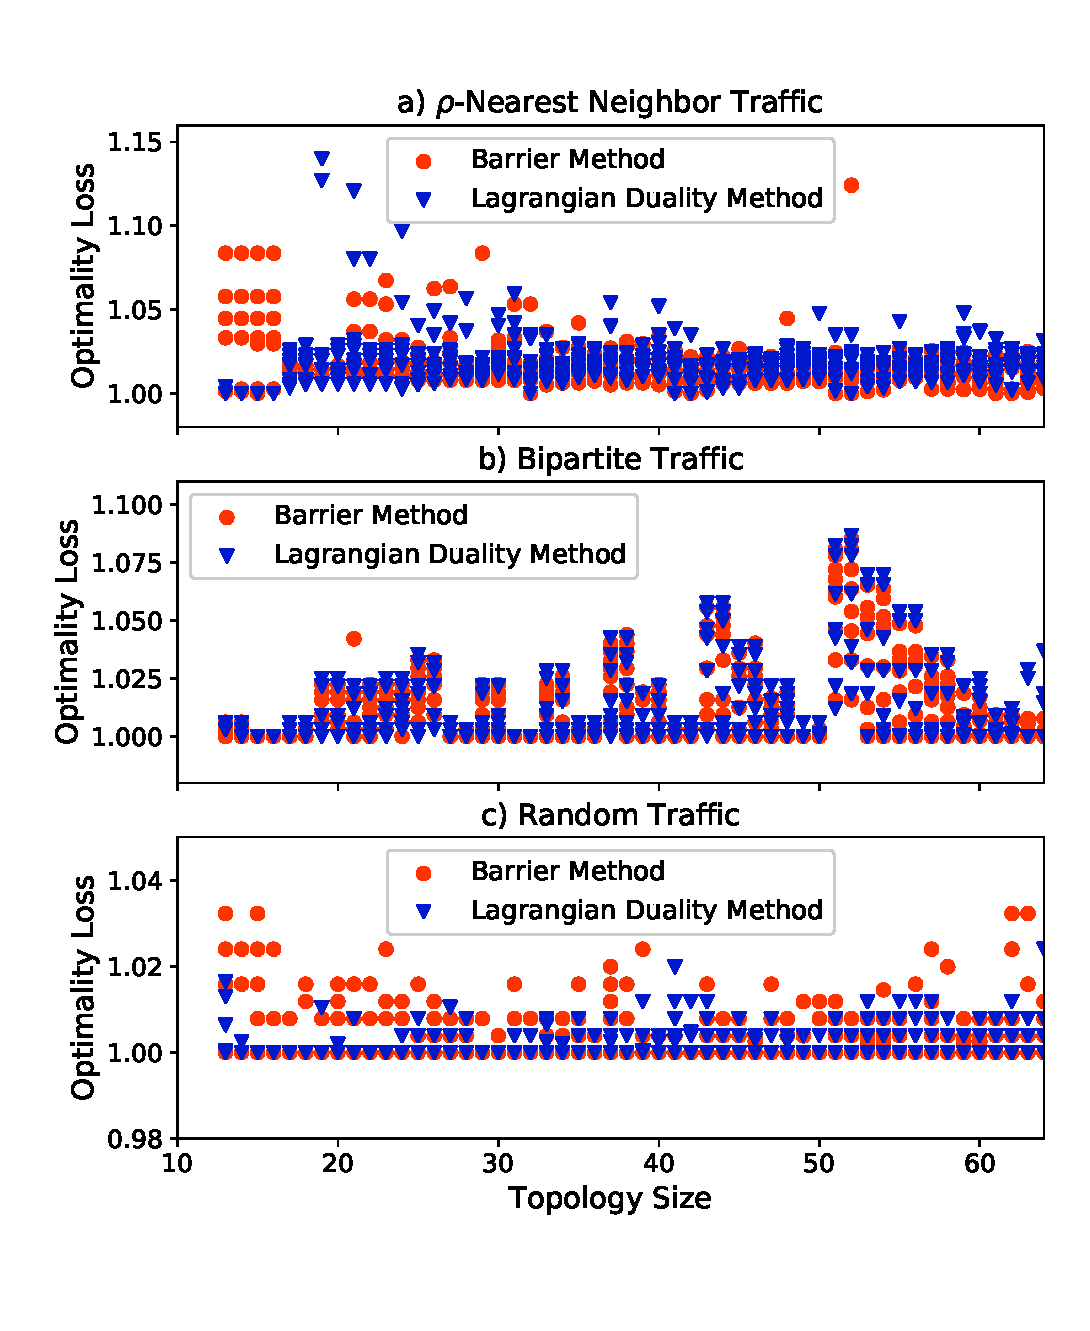
\includegraphics[trim={1cm 2.3cm 0.3cm 1.05cm},width=\linewidth,scale=1]{./figures/optimality_loss.eps}
    \caption{Benchmark on optimality loss for k-nearest neighbor, bipartite, and random traffic patterns}
    \label{optimality_loss_benchmark}
\end{figure}

\begin{figure*}[t]
    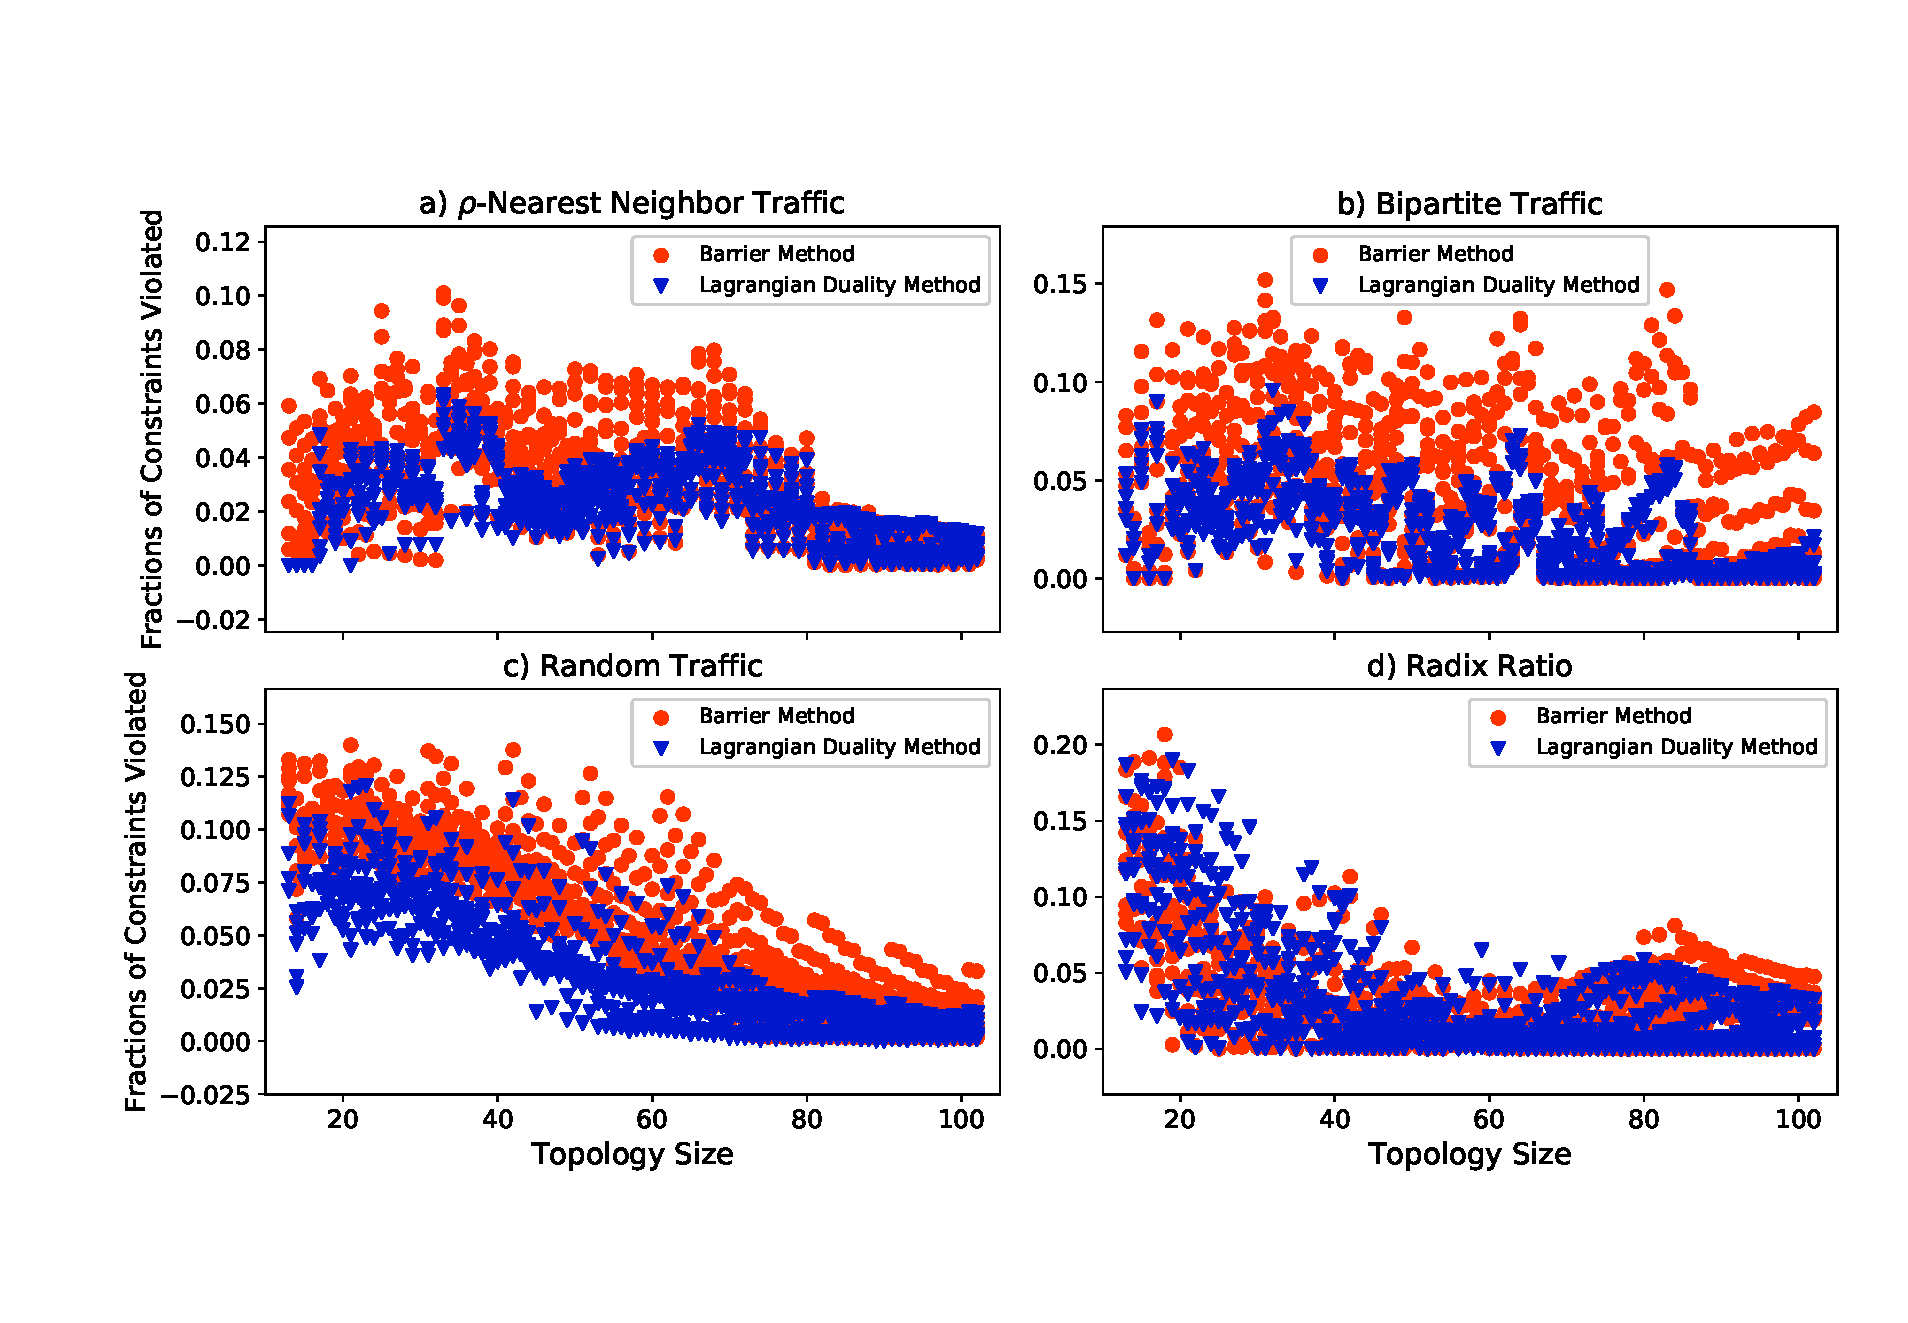
\includegraphics[trim={1cm 1.2cm 1cm 4cm}, width=1.\linewidth, height=8cm,scale=1.3]{./figures/constraints_violated.eps}
    \vspace{-1.3cm}
    \caption{Benchmark on fraction of constraints violated for 4 synthetic traffic patterns}
    \label{constraints_violation_benchmark}
\end{figure*}

\subsection{Runtime Analysis}
The runtime measured in seconds for both Lagrangian duality and barrier penalty methods running 50 iterations are shown in Figure \ref{runtime}. We noticed that while the exact runtime differs for different traffic matrices, the general trend is still similar with runtimes within the same order of magnitude. Therefore, we only show the runtime distribution as a function of fabric size under random traffic load. Note that in general, the barrier method is about twice as fast as the Lagrangian duality method. This speedup is likely linearized approximation of the objective function employed in the barrier method. Both methods completes within \~150s for even the largest fabric size with  >100 pods. These runtimes make both methods suitable for deployment within datacenters equipped with high speed optical switches. Under these conditions, the algorithms are able to map fractional topologies onto the optical switches at high-frequency. 
\begin{figure}[t]
    \centering
    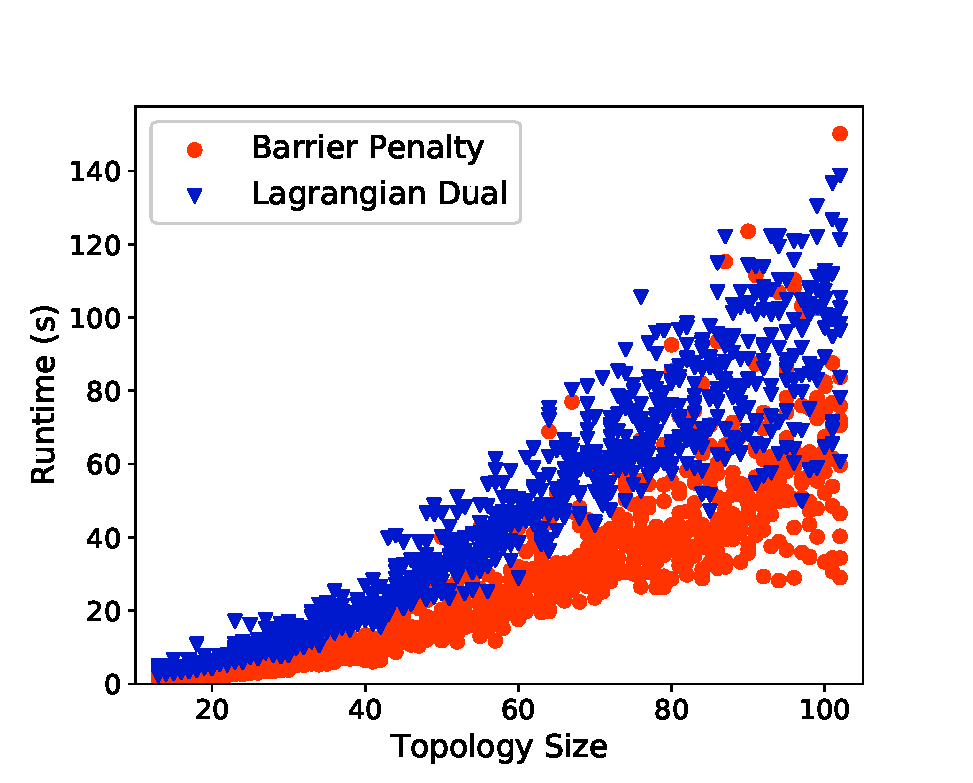
\includegraphics[height=7.5cm, width=\linewidth,scale=0.90, trim={0.7cm 0.7cm 1.5cm 0.8cm}]{./figures/runtime.eps}
    \caption{Runtime of both Lagrangian dual and barrier methods with $t_{max} = 50$}
    \label{runtime}
\end{figure}

\subsection{Barrier Penalty vs Lagrangian Dual}
In general, the Lagrangian duality method yields better optimality results and violates fewer matching constraints than the barrier penalty method, at the cost of a higher runtime. This higher runtime can be accredited to the Lagrangian dual method being complicated to implement in practice due to the introduction of its dual variables. The primal objective of the Lagrangian dual method we proposed does not seem to directly minimize matching constraint violation directly, as the constraints violation are only penalized indirectly through the introduction of the Lagrangian relaxation function. Interestingly, Lagrangian dual method has more adaptability due to the dual variables, through which the $\mathbf{p}^\pm$ variables and be updated in the iterative algorithm and help satisfy more constraints. The barrier method should in theory penalize constraint violation more harshly due to the quadratic nature of its objective function. However, it does not have the same kind of adaptability that the Lagrangian dual method has. 

We envision combining the best features of both methods through an Augmented Lagrangian Dual approach for future work. We posit that this approach could offer both adaptability through the dual variables, while penalizing matching constraints more harshly through higher-order barrier functions of the dual variables. Additionally, it may also be worth trying barrier penalty functions that penalizes over-provisioning of logical links between $(s_i, s_j)$ less severely than under-provisioning. This is because under-provisioning logical links between every may more negatively impact network congestion, especially when there is a significant amounts of traffic flowing through the $(s_i, s_j)$ links. That said, it is difficult to say that penalizing over-provisioning less may lead to better results. As is often the case in these NP-hard shared-resources \cite{irving1994three} problems, punishing an over-provisioned logical link less may result in the finite link resources being deprived to other under-provisioned inter-pod links. Nonetheless, these are ideas that are worth exploring in more detail in future literature.


\begin{figure*}[t!]
\centering
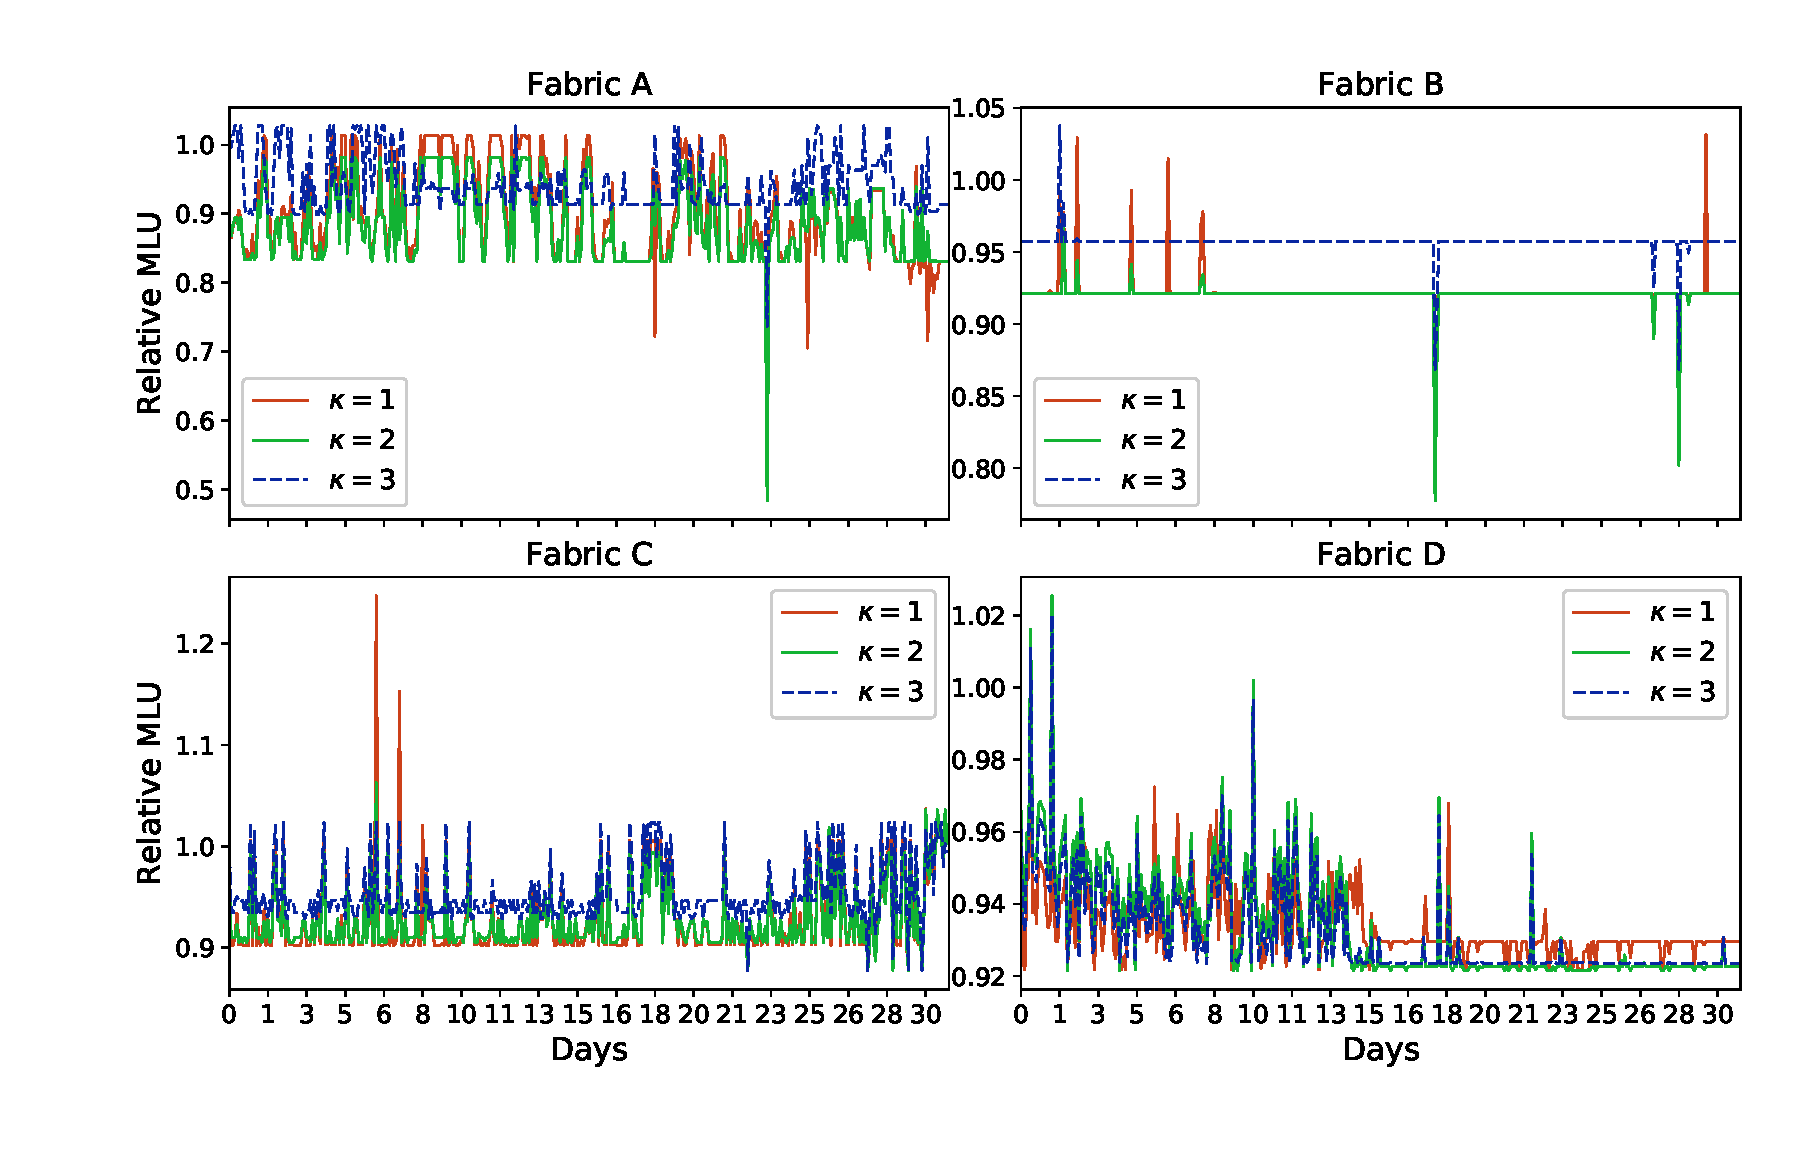
\includegraphics[scale=1.2, width=\textwidth, height=9cm, trim={2.5cm 1.9cm 1cm 0.85cm}]{figures/mlu.eps}
\caption{Month-long relative MLU performance with $\kappa = $ 1, 2, and 3.}
\label{mlu_results}
\end{figure*}

\section{Performance Evaluation}\label{section_timeseries_analysis}

\subsection{WCMP Traffic Engineering}   
Given a traffic matrix $T$ and a logical topology $\mathbf{x}$, we employ a two-hop, centralized WCMP \cite{zhou2014wcmp} routing with perfect traffic knowledge to for routing $T$ over topology $mathbf{x}$. Since we are solely interested in evaluating the quality of the logical topology, perfect traffic knowledge is assumed in order to reduce the impact of routing uncertainties on network performance metrics. The routing weights $w_p$ are derived using:

\begin{equation}\label{wcmp_routing}
\begin{aligned}
&\min\limits_{\eta, \boldsymbol{\omega_p}} \; \quad \eta \\
\text{s. t: } & 1) \; \sum_{p \in P_{ij}} \omega_{p} = t_{ij} \quad \forall \; i, j \in S\\
& 2) \; \sum_{p \in P(e_{ij})} \omega_p \leq \eta \; b_{ij} \sum_{k \in O}x_{ij}^k \quad \forall \; i, j \in S \\
\end{aligned}
\end{equation}

Where $\eta$ denotes the max link utilization, while $\omega_p$ denotes WCMP weight allocated to path $p$. Constraint 1 in (\ref{wcmp_routing}) states that the WCMP weights through all paths between $s_i$ to $s_j$ to equal the traffic flow from $s_i$ to $s_j$, ensuring that the routing has to ensure that all traffic flows have to reach their intended destinations. Constraint 2 enforces all inter-pod link utilizations to be bounded by the max link utilization. Note that (\ref{wcmp_routing}) is essentially traffic engineering, with the objective of minimizing maximum congestion.


\subsection{Performance Metrics \& Experimental Setup}
% first, briefly talk about the experimental setup
In our experiments, we simulate the effects of traffic-aware topology engineering on 4 production data-centers using real historical traffic data. Since our evaluations are based on real traffic data, it is very natural to use link-utilizations to measure the network performance. These metrics are computed hourly over a month-long duration. The network performance of the same traffic are also evaluated on uniform topologies that only use traffic engineering, as described in (\ref{wcmp_routing}) for link load-balancing. The evaluated metrics are:

\begin{itemize}
    \item \textbf{Relative Max Link Utilization (MLU)}
    \item \textbf{Relative 90-th Percentile Link Utilization (LU90)}
    \item \textbf{Stretch Factor (SF)}
\end{itemize}

Link utilization measures the ratio of traffic flowing over a link to its bandwidth, and max link utilization simply the most highly utilized link within the network under a given traffic load. In addition to measuring MLU, which is a good proxy for maximum network link congestion, we also measure the 90-th percentile link utilizations to get a sense of how quickly the link congestion distribution decays. To show the relative impact on link congestion introduced by traffic-aware topology engineering and to anonymize traffic data, we normalize using the link utilization metrics measured using a baseline uniform topology, and call these metrics relative link utilizations.

Additionally, we also compute the stretch factor hourly using $\frac{\sum\limits_{p \in P}l_p \omega_p}{\sum \limits_{p \in P}\omega_p}$. Stretch factor represents the average hop count for each unit of traffic, and is a useful proxy for estimating the per-packet delay. Since we are using two-hop routing, the stretch factor should lie between 1 and 2.


\begin{figure*}[t!]
\centering
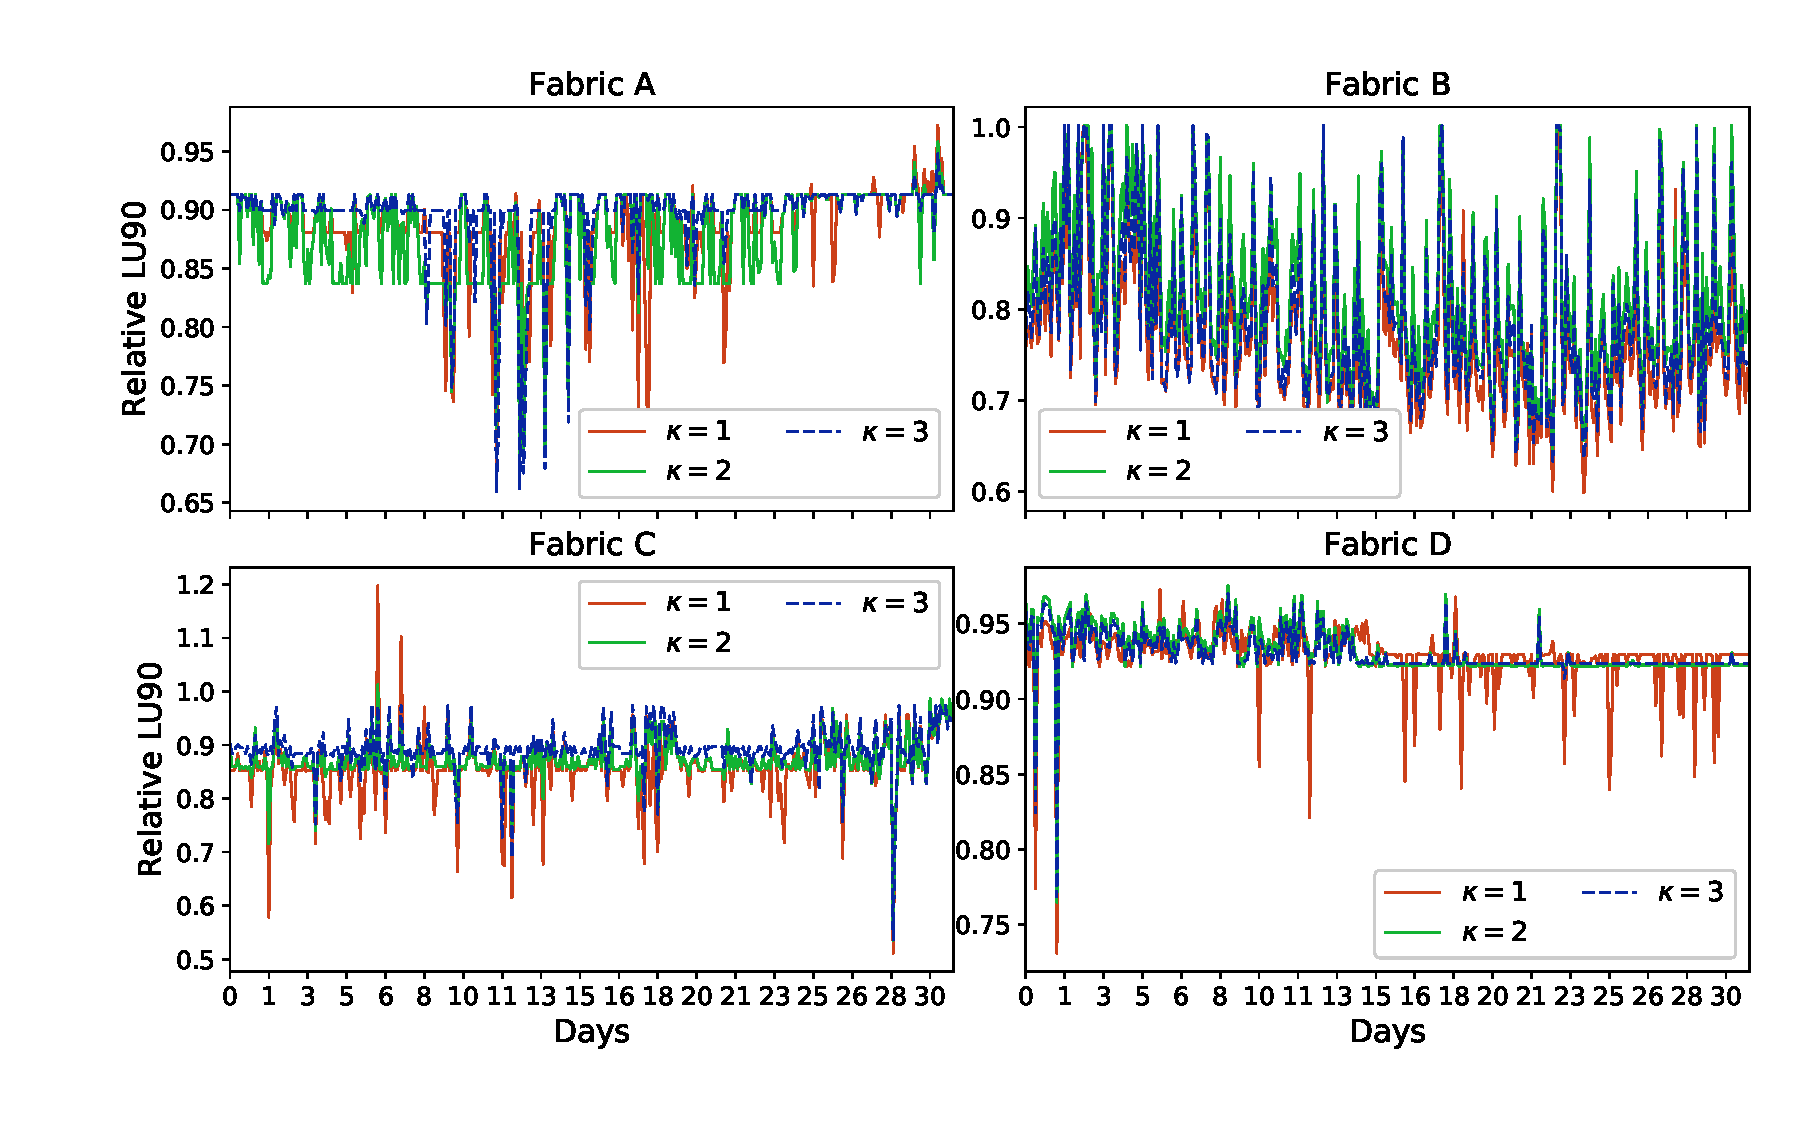
\includegraphics[scale=1.2, width=\textwidth, height=9cm, trim={2cm 1.9cm 1cm 0.60cm}]{./figures/lu90}
\caption{Month-long relative LU90 performance with $\kappa = $ 1, 2, and 3.}
\label{lu90_results}
\end{figure*}

\subsection{Discussion}
Figure \ref{mlu_results} shows the relative MLU performance using topology designed from 1 to 3 traffic clusters. Results in all 4 fabrics show that for most time slots, picking $\kappa = 1$ is sufficient and outperforms $\kappa = 2, 3$. This makes sense, as factoring in more traffic matrices in the topology engineering process not just complicates the model, it also tends to render the topology less optimal for any single traffic matrix. Fabric D shows the usefulness of considering multiple traffic matrices in topology engineering, as the links become noticeably less congested past day 13, indicating that shifted traffic patterns cannot not be accounted for picking just 1 cluster. In fabrics B and C, sporadic significant MLU degradation occur when $\kappa = 1$ but not when $\kappa = 2, 3$. These instances further highlights the need for accounting for multiple traffic-matrices when performing topology engineering to render the topology more robust to potential significant traffic pattern changes. 

Figure \ref{lu90_results} shows the relative LU90 measurements. Here we can see clearly that LU90 improves rather significantly using topology engineering, since more links can be allocated between pod pairs with higher traffic flows. As such, more traffic can take direct-hop paths to reach their destination without driving up the link congestion levels. This is not possible in a uniform topology, since keeping the link congestion levels low would often imply sending traffic via non-minimal paths, therefore generating more network traffic and driving up the average and percentile link congestions.

In addition to link congestion, the performance improvements enabled by using our propose methodology becomes much clearer when measuring the stretch factor, as shown in Figure \ref{stretch_factor_results}. Here we can see that for all 4 fabrics, almost all of the traffic are allocated to single-hop paths. Besides lowering the average link congestion levels, the lower average hop count implies that the average time a packet spends within the network is less as a result of taking a direct path to its intended destination. This makes topology engineering ideal for improving performances of more latency-sensitive applications. 

Our results also points out the inadequacies of traffic engineering alone, since traffic engineering relies trades link de-congestion for increased average hop-count (and thus average packet latency). In fact, the stretch-factor and maximum link congestion are often times mutually-exclusive, since reducing link congestion might require the routers to divert traffic along non-minimal paths. We emphasize that a traffic-aware topology-engineering methodology solves both these issues at once.


\begin{figure*}[ht]
\centering
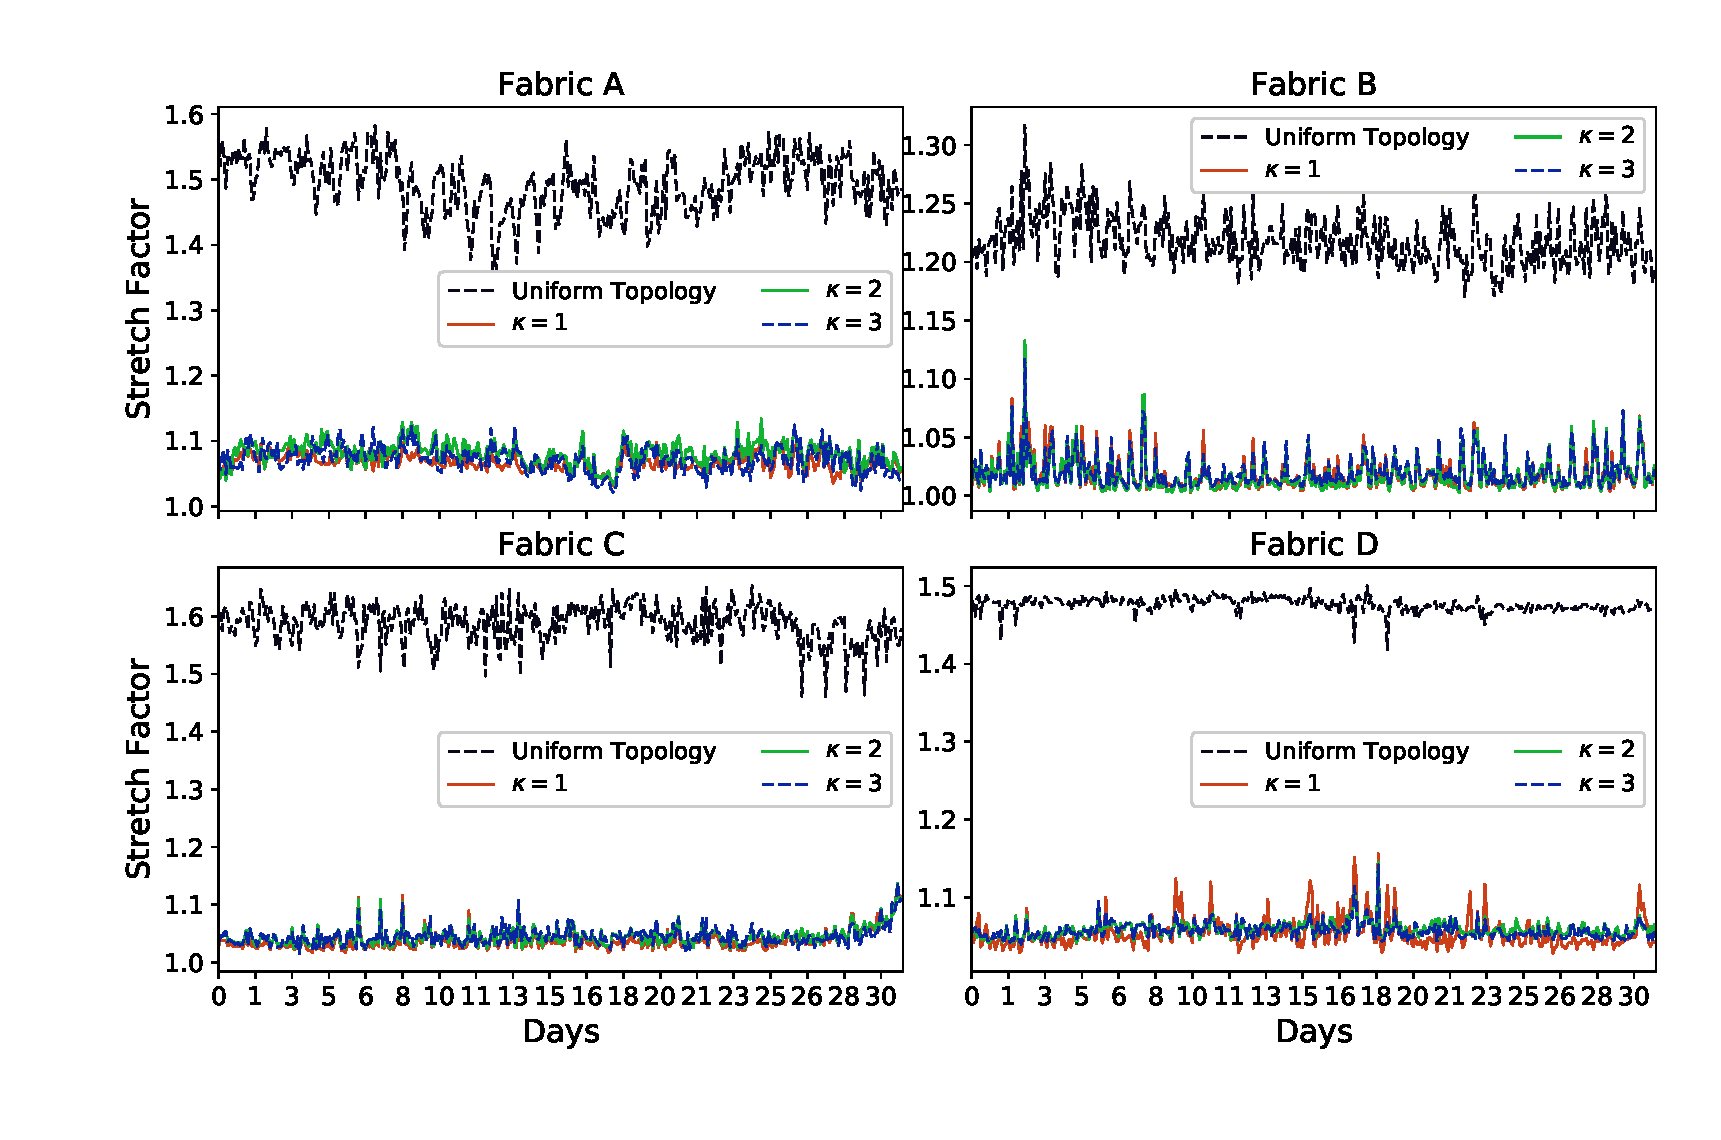
\includegraphics[scale=1.2, width=1.03\textwidth, height=9cm, trim={2cm 1.9cm 0cm 0.6cm}]{figures/stretch_factor.eps}
\caption{Month-long stretch factor performance with $\kappa = $ 1, 2, 3, and uniform topology.}
\label{stretch_factor_results}
\end{figure*}

\section{When to Trigger Topology Reconfiguration}\label{section_when_to_reconfigure}
One potential issue of our approach is that as traffic modes begin to change, it is likely that the network will begin to suffer performance degradation. Therefore, the general rule of thumb is that the entire pipeline shown in Figure \ref{topology_engineering_overall_workflow} should be triggered whenever traffic modes begin to demonstrably change. Events that lead to drastic changes in long-term traffic pattern tends to arise when these is a major DCN expansion. A new logical topology should be computed whenever there is a DCN expansion. Adding new pods into the network can significantly affect the traffic modes. In addition, topology reconfiguration should be triggered when there is a link upgrade for any pod within the network, sicne the . Sometimes, the network performance can degrade over time as the underlying production areas change. A change in production area can upset the traffic modes tremendously, since the different applications can exhibit vastly different network traffic behavior. In general, topology reconfiguration should be triggered whenever there is a change in this . 

To reduce the frequency of topology reconfiguration, we need to work on desensitizing the network performance change as traffic modes exhibit drastic changes. This is an ongoing work for us, and thus will be treated more rigorously in future works. 


\section{Conclusion}\label{section_conclusion}
%We propose a traffic-aware topology design methodology based on the co-optimization of both the logical topology and the routing. We've proposed a robust and fast logical topology reconfiguration algorithm by While our proposed methodology is aimed at monthly-reconfiguration, the topology reconfiguration algorithm can is fast and can be used for real-time reconfiguration. In other words, the topology reconfiguration algorithm can be employed within datacenter and even HPC networks that utilize optical switching with faster reconfiguration time.

%% we depart from established literatures tackling reconfigurable topology by noticing that traffic have frequently-occuring modes. With this we propose a robust reconfigurable topology scheme that optimizes for multiple traffic matrices 
We propose a traffic engineering methodology with that does not require traffic-prediction. By considering multiple persistent traffic modes that can be derived using historical traffic matrices, our topology engineering solution proves robust under traffic change for long periods of time compared to uniform topologies that rely solely on traffic engineering for network load-balancing. Most importantly, we do not rely on sophisticated and immature circuit-switching hardware, therefore can be readily deployed in today's DCN equipped with cheap commodity patch-panels. Our experimental results using production traffic show that our topology engineering methodology can reduce maximum link congestion, while also keeping most traffic within one-hop. We believe that for future works, different clustering techniques can be looked into in order to select more representative traffic matrices. Similarly, many different methods of mapping a computing logical topology and map it onto a non-fully connected network can should be looked into.



%%\input{./figures/min_cost_flow_bipartite.tex}
\bibliographystyle{ACM-Reference-Format}
\clearpage
\bibliography{reference}
% Uncomment the following lines if we choose to include appendices
%\newpage
\clearpage
\clearpage
\begin{appendices}

\section{Appendices}
\subsection{Simplex-based Patch Panel Reconfiguration}
In mapping the fractional graph to the patch-panels such that the logical topology looks identical to the the fractional graph. We consider the logical topology as being identical to the fractional demand if $\sum_{k \in O}x_{ij}^k \leq c_{ij}^+$ and $\sum_{k \in O}x_{ij}^k \geq c_{ij}^-$. To find the integer solution to this SAT problem is NP-hard in general, therefore we employ an LP-relaxation of the SAT-problem. The SAT problem is rewritten as a linear program as follows:
\begin{equation}\label{simplex}
\begin{aligned}
    & \max 0\\
     \text{s. t} & \quad (\ref{phy_constraint1}), \; (\ref{phy_constraint2}), \; (\ref{con_constraint})\\
\end{aligned}
\end{equation}
This algorithm relies on the simplex method's natural propensity to produce integer solutions, as the pivoting algorithm iteratively searches the optimal solutions on the polytope vertices. Conveniently, the vast majority of integer solutions to (\ref{simplex}) do conveniently lie on the vertices, laying well within the simplex algorithm's search space. For the remaining non-integer solutions, we round them into integers using min-cost flow with the the arc-weights of $\ceil{x_{ij}^k {}^*} - x_{ij}^k{}^*$.

While certainly intuitive, this method does not work well with the fractional graph optimization derived in for all permutations of traffic matrices. We've tried this method using a variety of fractional graph permutations that are non-uniform and noted that in most cases, a the simplex algorithm crashes due to the inability to find a feasible solution. Since this method breaks down when there is no feasible solution to the SAT problem, it is not suitable for deployment for all permutations of the fractional graph. The simplex method also does not scale well to larger problem sizes due to a significant runtime increase. In fact, the simplex method has a provable exponential worst-case runtime makes this method not robust enough for deployment in real systems.


\subsection{Topology Engineering Benefits}
We consider 2-hop routing so as to allow some the network to load-balance through routing. Consider the following example:

%%Draw the 4 point graph and dummy example with mlu improvement by 50% with topology engineering, and claim that it generalizes to varying degrees of improvement for M-to-N bipartite communications

We posit that there are certain traffic patterns under which traffic-aware topology design will prove most useful. One such example is a $M$-to-$N$ bipartite traffic pattern, whereby each of the $M$ senders send traffic to all $N$ receivers. These traffic are expected to arise when datacenter architectures become increasingly disaggregated, where there are $M$ pods with purely compute resources that need to write data into storage distributed across $N$ storage pods. To clarify this concept, we present the following example.

Consider a datacenter network with 2 sets of pods $A = \{a_1, a_2, ..., a_n\}$ and $B = \{b_1, b_2, ... , b_n\}$, whereby the set of all pods is given as $S = A \cup B$. The network topology is that of an all-to-all with a uniform link capacity of $c$. Suppose we have the traffic demand described by:
\begin{equation}
\begin{aligned}
    t_{ij} = \begin{cases}
                \alpha, \text{ if } a_i \in A \text{ and } b_j \in B\\
                0, \text{ otherwise}
    \end{cases}
\end{aligned}
\label{eqn:bipartite_traffic}
\end{equation}
We assume 2-hop routing for network load-balancing, and every node can be used as an intermediate hop. Using the available uniform topology shown in Figure \ref{uniform_topology}, the max link utilization with perfect load balancing is $\frac{(2n-1)\alpha}{c}$. Using traffic-aware topology design, however, we can disconnect the $n - 1$ links that each sender in $A$ to other sender nodes in the same set, and connect them to $n - 1$ receivers in set $B$ instead, resulting in the topology shown in Figure \ref{traffic_aware_topology}. In this case, the max link utilization under perfect load-balancing is $\frac{n \alpha}{c}$. This shows that with traffic-aware topology designs we can reduce max link utilization to a factor of $\frac{n}{2n - 1} \approx \frac{1}{2}$ than that obtained form traffic-agnostic topologies.
\begin{itemize} 
    \item \textbf{Singular hotspot} - When one pod sends or receives significantly more traffic than all of its peers, the most congested links will be located at either the egress or ingress links of said pod. Topology engineering cannot alleviate bottlenecks due to physical bandwidth limitations.
    \item \textbf{Uniform traffic} - Under a uniform traffic load, there is no need for special topology design. The ideal topology to handle a uniform traffic pattern is a uniform one.
\end{itemize}

\begin{figure}
\centering
\begin{tikzpicture}[->,>=stealth',shorten >=1pt,auto,node distance=1.4cm,
                    thick,main node/.style={circle,draw,font=\sffamily\Small\bfseries}, scale=0.7]

  \node[main node] (1) {$a_1$};
  \node[main node] (2) [right of=1] {$a_2$};
  \node[main node] (3) [right of=2] {$a_3$};
  \node[main node] (4) [right of= 3, xshift=1cm] {$a_n$};
  \node[main node] (5) [below of=1] {$b_1$};
  \node[main node] (6) [below of=2] {$b_2$};
  \node[main node] (7) [below of=3] {$b_3$};
  \node[main node] (8) [below of=4] {$b_n$};
  
  \node at ($(3)!.5!(4)$) {\ldots\ldots};
  \node at ($(7)!.5!(8)$) {\ldots\ldots};
  
  \path[every node/.style={font=\sffamily\small}]
    (1) edge node [left] {$c$} (5)
        edge node[left] {} (6)
        edge node [left] {} (7)
        edge node [left] {} (8)
        edge node [-] {} (2)
        edge [bend left] node [bend left] {} (3)
        edge [bend left] node [left] {$c$} (4)
    (2) edge node [left] {} (5)
        edge node [left] {} (6)
        edge node [left] {} (7)
        edge node [left] {} (8)
    (3) edge node [right] {} (6)
        edge node [right] {} (7)
    (4) edge node [right] {} (6)
        edge node [left] {} (5);
\end{tikzpicture}
\caption{Uniform topology}
\label{uniform_topology}
\end{figure}

\begin{figure}
\begin{tikzpicture}[->,>=stealth',shorten >=1pt,auto,node distance=1.4cm,
                    thick,main node/.style={circle,draw,font=\sffamily\Small\bfseries}]

  \node[main node] (1) {$a_1$};
  \node[main node] (2) [right of=1] {$a_2$};
  \node[main node] (3) [right of=2] {$a_3$};
  \node[main node] (4) [right of= 3, xshift=1cm] {$a_n$};
  \node[main node] (5) [below of=1] {$b_1$};
  \node[main node] (6) [below of=2] {$b_2$};
  \node[main node] (7) [below of=3] {$b_3$};
  \node[main node] (8) [below of=4] {$b_n$};
  
  \node at ($(3)!.5!(4)$) {\ldots\ldots};
  \node at ($(7)!.5!(8)$) {\ldots\ldots};
  
  \path[every node/.style={font=\sffamily\small}]
    (1) edge node [left] {$2c$} (5)
        edge node[left] {} (6)
        edge node [left] {} (7)
        edge node [left] {} (8)
    (2) edge node [left] {} (5)
        edge node [left] {} (6)
        edge node [left] {} (7)
        edge node [left] {} (8)
    (3) edge node [right] {} (6)
        edge node [right] {} (7)
    (4) edge node [right] {} (6)
        edge node [left] {} (5);
\end{tikzpicture}
\caption{Traffic-aware topology for bipartite traffic} \label{traffic_aware_topology}
\end{figure}


\subsection{Correctness of Minimum-cost Circulation}\label{appendix:mincost_flow}
%% write down how a patch-panel is modeled as a bipartite flow graph with dummy source and destination, and how the min cost flow's arc costs are given, and how the upper bound of each flow and the lower bounds are enforced
\begin{figure}[ht!]
    \centering
    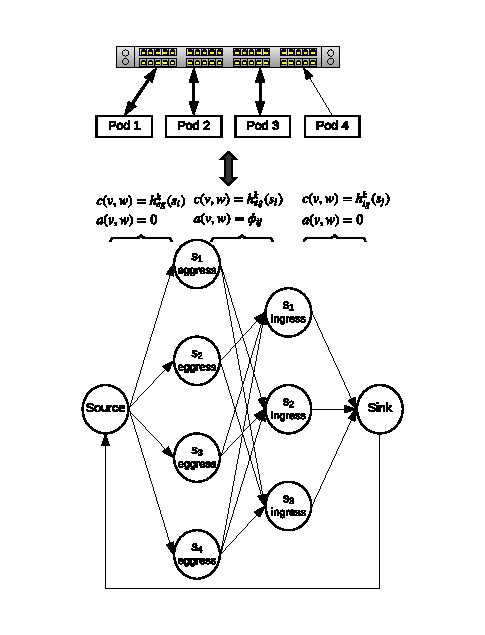
\includegraphics[width=2.5in,height=3.8in,trim={1.3cm 0.6cm 1.3cm 0cm}]{./figures/mincost_circulation_mapping}
    \caption{Mapping a patch panel's physical striping onto a network flow graph}
    \label{fig:mincost_circulation_mapping}
\end{figure}
Here we prove that the integer optimization of equations (\ref{primaldual_linear_approx}, \ref{barrier_linear_approx}) is equivalent to a min-cost circulation problem. For any min-cost flow problem, the objective is to find a flow assignment $f(u,v)$ that minimizes:
\begin{equation}
\begin{aligned}
&\min \sum\limits_{(v, w) \in E} f(v,w) \cdot a(v,w)\\
\text{s.t } & 1) \; l(v, w) \leq f(v, w) \leq \min\big(u(v,w), c(v,w)\big)\\
            & 2) \; \sum\limits_{u \in V} f(u, v) = \sum\limits_{w \in V} f(v, w) \; \forall \; v \in V \\ 
\end{aligned}\label{equation:min_cost_circulation_theoretical}
\end{equation}
Where $a(u, v)$ and $c(v,w)$ denote the cost per unit flow and capacity for the $(u,v)$ edge, respectively. The first constraint sets the closed range between which the flow must lie without violating the capacity constraint of each edge, while the second constraint is simply a enforces flow-conservation on any node that is neither the source nor sink node. To prove, we begin by illustrating how a flow digraph, $G_k= (V, E)$, for patch panel $k$ is generated based on its physical striping. Using this mapping, $f(s_i, s_j)$ is equivalent to $x_{ij}^k$.

First, we prove that a solution which satisfies constraints in (\ref{equation:min_cost_circulation_theoretical}) also satisfies (\ref{primaldual_linear_approx}) and (\ref{barrier_linear_approx}). We know that the flow from each egress vertex satisfies constraint 1 in (\ref{equation:min_cost_circulation_theoretical}), therefore the following inequality is true: $\sum\limits_{i \in S} f(s_i, s_j) \leq h_{ig}^k(s_j) \; \forall \; j \in S$. Similarly, since we've capped the flow capacity of each arc from the dummy source vertex to the ingress vertices by $h_{eg}^k(s_i)$, we can be certain that a flow that satisfies constraint 1 in (\ref{equation:min_cost_circulation_theoretical}) is guaranteed to to satisfy the inequality: $\sum\limits_{j \in S} f(s_i, s_j) \leq h_{eg}^k(s_i) \; \forall \; i \in S$. Meanwhile, constraint 2 of (\ref{equation:min_cost_circulation_theoretical}) is simply a flow conservation constraint for the Min-cost Circulation problem and has no relation to problems (\ref{primaldual_linear_approx}) and (\ref{barrier_linear_approx}).

Next, we prove that an optimal solution to (\ref{equation:min_cost_circulation_theoretical}) is also optimal for (\ref{primaldual_linear_approx}) and (\ref{barrier_linear_approx}). Since $a(v,w) = 0$ for all arcs that either originates from or leads toward the dummy source and sink nodes, respectively, the objective function for the min-cost flow problem reduces to $\sum\limits_{i, j \in S} f(s_i, s_j)\phi_{ij}$. Therefore, a solution that minimizes this reduced form also minimizes (\ref{primaldual_linear_approx}) and (\ref{barrier_linear_approx}).

%\begin{comment}

%% we want to prove that the solution from min-cost circulation will definitely satisfy the constraints of striping
%\end{comment}


%\subsection{Complete Lagrangian Dual Derivation}
%\input{./sections/appendix/detailed_lagrangian_duality_derivation.tex}

\subsection{Alternative Fractional Graph Computation}
In this section, we detail a routing-topology co-optimization methodology used for computing an optimal fractional topology given a set of traffic matrices. As mentioned briefly in Section \ref{section_challenges_overall_approach}, we've decided to tackle the optimal logical topology computation by splitting the large problem into two smaller, more easily-solvable problems. In computing the optimal topology, we've decided to ignore the patch panel layer and assume full-connectivity, which is motivated by two reasons: Firstly, considering the patch-panel layer increases the number of variables and constraints required to formulate the LP, which incurs scalability issues when optimizing for larger topologies. Secondly, including the patch-panel layer (which will be considered in Step 3 regardless) brings about negligible improvement (if any) to the optimality of our final integer logical topology. 

Step 2 of Figure \ref{topology_engineering_overall_workflow} shows that instead of considering all traffic modes in the same fractional derivation computing, we compute a fractional topology optimal for each traffic mode, and then finally combine all these topologies using LP. This is because formulating an LP that considers all the traffic modes together greatly increases the complexity of the problem. Based on our experience, solutions obtained from LP's tend to be unstable, therefore we employ a quadratic program (QP) to stabilize the fractional topology for each traffic mode. Finally, all the $\kappa$ fractional topologies are linearly combined using LP.

Given that we assume full-connectivity here, the only physical constraints to be imposed for computing fractional topologies are:
\begin{equation}
\sum\limits_{j \in S} d_{ij} \leq r_{eg}^i \; \forall \; i \in S 
\label{constraint:egress}
\end{equation}
\begin{equation}
\sum\limits_{i \in S} d_{ij} \leq r_{ig}^{ j} \; \forall \; j \in S
\label{constraint:ingress}
\end{equation}
Constraints (\ref{constraint:egress}) and (\ref{constraint:ingress}) upper-bounds the number of links formed by $s_i$ with its peer pods to its total number of egress links and ingress links, respectively. Now, given a traffic mode $T^\kappa$, we want to obtain an fractional topology that can support the largest scale-up of $T^\kappa$ under multihop routing, which can be formulated as the following LP:

\begin{equation}
\begin{aligned}
 & \max\limits_{\mu_\kappa, \boldsymbol{\omega_p}, \mathbf{d}} \; \quad \mu_{\kappa} \\
\text{s. t: } & 1) \; \sum_{p \in P_{ij}} \omega_{p} = \mu_{\kappa} \; t_{ij}^k, \quad \forall \; i, j \in S \\
& 2) \sum_{p \in P(e_{ij})} \omega_{p} \leq d_{ij} b_{ij}, \; \forall \; i, j \in S\\
& 3) \quad (\ref{constraint:egress})\; , \; (\ref{constraint:ingress})
\end{aligned}\label{fractional_graph_lp}
\end{equation}
Where $b_{ij} = \min(b_i, b_j)$ and $\mu_{\kappa}$ is the traffic matrix scale-up factor for traffic mode $\kappa$. Constraint 1 enforces all scaled-up $i$ to $j$ traffic demands to be satisfied via all routable paths, while constraint 4 ensures that the traffic flowing through each link cannot exceed its bandwidth. Unfortunately, the linear nature of (\ref{fractional_graph_lp})'s objective function causes the solution to suffer from stability issues. (\ref{fractional_graph_lp}) implies that there may be many different fractional topologies that can support the same scale-up factor, $u^\kappa$, with some viable fractional topologies perhaps relying more heavily on multi-hop routing rather than direct-hop routing. We know that relying on multi-hop routing not just increases the delay of each packet, but could also inadvertently congest other network links as overall traffic increases. To solve this issue, we extract the each traffic mode's maximal scale-up factor, $\mu_\kappa^{*}$, by solving (\ref{fractional_graph_lp}). Using the computed scale-up factor, we stabilize the fractional topology solution using a the strongly-convex properties of a quadratic program (QP) with linear constraints that acts as a solution ``filter''. So, for each traffic mode, the objective of this quadratic program is set to minimize multi-hop routing as much as possible while still supporting the same scale-up factor:
\begin{equation}
\begin{aligned}
\min\limits_{\boldsymbol{\omega_p}, \mathbf{d}} \;& \quad \sum_{i, j \in S} \; \sum_{p \in P_{ij}(l_p > 1)}\big(\omega_{p}\big)^2 \\
\text{s. t: } & 1) \; \sum_{p \in P_{ij}} \omega_{p} = \mu_{\kappa}^* t_{ij}, \quad \forall \; i, j \in S \\
& 2) \sum\limits_{p \in P(e_{ij})} \omega_{p} \geq \mu_{\kappa}^* \; d_{ij} b_{ij}, \quad \forall \; i, j \in S\\
& 3) \quad (\ref{constraint:egress}) \; , \; (\ref{constraint:ingress})
\end{aligned}\label{fractional_graph_qp}
\end{equation}
Where $P_{ij}(l_p > 1) = \{p \; | \; p \in P_{ij} \cap l_p > 1\}$ denotes the set of routing paths from $s_i$ to $s_j$ with hop-counts greater than 1. To solve (\ref{fractional_graph_qp}), we use the OSQP library \cite{osqp}. By attempting to minimize multihop routing, (\ref{fractional_graph_qp}) indirectly forces the fractional topology to ``match'' the traffic matrix. This has the added benefit of making the $\kappa$-th traffic mode's fractional topology to remain fairly optimal for traffic matrices that fall within mode $\kappa$'s cluster.

With each traffic mode, $T^\kappa$'s stable fractional topologies computed, we combine them into one fractional topology using linear combination of the form:
\begin{equation}
\begin{aligned}
 & \max\limits_{\alpha, \mathbf{d}^*} \; \quad \alpha \\
 \text{s. t: } & 1) \quad d_{ij}^* \geq \; \alpha \; d_{ij}^\zeta, \; \forall \; i, j \in S, \; \zeta \in \{1, 2, ..., \kappa\} \\
  & 2) \quad (\ref{constraint:egress}) \;, \; (\ref{constraint:ingress})
\end{aligned}\label{combine_fractional_graphs}
\end{equation}
Where $\alpha$ is the scaling factor of each individual fractional graph. Constraint 1 in (\ref{combine_fractional_graphs}) is imposed so that each $(i, j)$ fractional link in the combined fractional graph, $d_{ij}^*$, can dominate all other $\alpha$-scaled $d_{ij}^\zeta \; \forall \; \zeta \in \{1,2, ..., \kappa\}$.

Here we define fractional topology a little more rigorously. A fractional topology describes the number of link counts between two pods in the topology. As its namesake suggests, the number of links between two pods . More concretely, a fractional topology can be described using a matrix, where the entry in $(i,j)$ denotes the fractional number of links connecting the egress ports of $s_i$ to the ingress ports of $(s_j)$. In addition, a fractional topology has to satisfy the degree constraints:

Furthermore, for any pair of $T$ and $D$, we consider $(T, D)$ feasible there a
\begin{equation}
\begin{aligned}
\min\limits_{\boldsymbol{\omega_p}, \mathbf{d}} \;& \quad \sum_{i, j \in S} \; \sum_{p \in P_{ij}(l_p > 1)}\big(\omega_{p}\big)^2 \\
\text{s. t: } & 1) \; \sum_{p \in P_{ij}} \omega_{p} = \mu_{\kappa}^* t_{ij}, \quad \forall \; i, j \in S \\
& 2) \sum\limits_{p \in P(e_{ij})} \omega_{p} \geq \mu_{\kappa}^* \; d_{ij} b_{ij}, \quad \forall \; i, j \in S\\
\end{aligned}\label{eqn:feasible_fg}
\end{equation}


\subsection{Effects of Applying QP ``filter''}
In (\ref{fractional_graph_qp}), minimizing the WCMP weights placed on multi-hop paths indirectly increases the weights placed on direct-hop paths under a given traffic matrix, subject to the constraint that the resulting traffic matrix scale-up factor, $\mu^*$, is preserved. Here, we show the utility for (\ref{fractional_graph_qp}) using the following Figure \ref{fig:qp_filter_vs_no_filter}, and discuss potential implications if a QP filter isn't employed.

\begin{figure}[ht!]
    \centering
    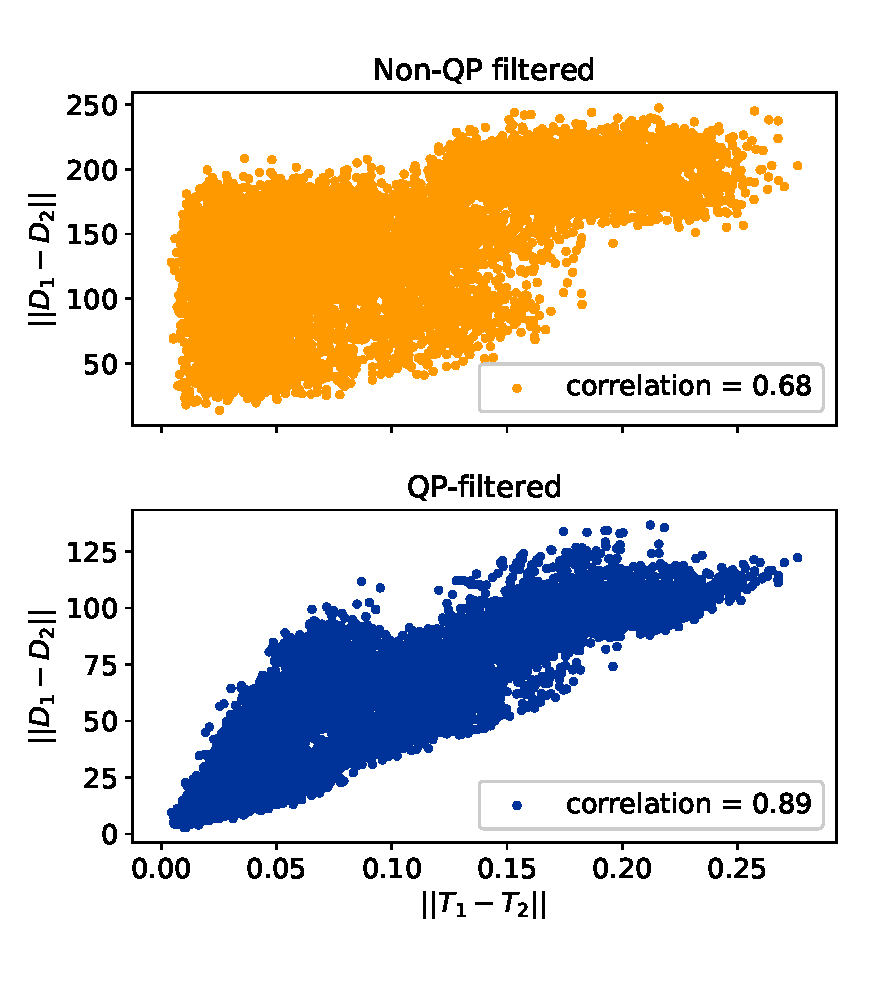
\includegraphics[width=2.5in,height=3.1in,trim={1.7cm 1.5cm 1.7cm 0.6cm}]{./figures/qp_filter_corr.eps}
    \caption{Mapping a patch panel's physical striping onto a network flow graph}
    \label{fig:qp_filter_vs_no_filter}
\end{figure}
In Figure \ref{fig:qp_filter_vs_no_filter}, the x-axis denotes the euclidean distance between two traffic matrices, while the y-axis denotes the euclidean distance between the computed fractional topologies for the corresponding traffic matrices. The traffic matrices are obtained from historical production DCN traffic.

Observing the two scatter plots in Figure \ref{fig:qp_filter_vs_no_filter}, it is clear that the QP-filter is doing a good job at producing fractional topology that matches the traffic matrix, as demonstrated by the strongly positive correlation of 0.89. Meanwhile, the non-QP-filtered fractional topology demonstrate a significantly poorer correlation between traffic matrix distance and resulting optimal fractional topology closeness. In fact, for the Non-QP filtered case, the spread of fractional topology distance when traffic matrix distance is close to 0 is rather significant. This spread is due mainly to 2 reasons: 1) there can be many different fractional topologies that could support the same traffic matrix scale up factor, $\mu^*$, with some perhaps utilizing more indirect-hops, and 2) the fractional topology solution given the same traffic matrix obtained from a LP solver is non-deterministic, and depends on the implementation of said solver. As such, employing a QP-filter in as much as an attempt to pick a fractional topology that maximizes direct-hop routing from a set of fractional topologies that could all support the same $\mu$, as it is an effort of reducing the solution oscillation obtained directly from a LP solver.

Most importantly, employing a QP filter helps ensure the fractional topology we compute for a traffic cluster is likely going to be quite optimal for traffic matrices that are in close proximity to the clusters. This has an effect of helping the fractional topology designed from a traffic mode to be able to handle many traffic matrices that exhibit very slight variation from said mode.

%% introduce the concepts of quadratic program matching

\subsection{Synthetic Traffic Generation}
\subsubsection{Bipartite\\}
The basic idea of the bipartite traffic is to emulate a potential traffic pattern that could arise as data center desegregates compute resources from their storage resources. Since the bipartite traffic pattern is given in (\ref{eqn:bipartite_traffic}), we will not repeat the equation here.

\subsubsection{$\kappa$-Nearest Neighbor\\}
With this traffic pattern, we attempt to emulate the traffic pattern where pods only send traffic to it's closest peers using circular distance. This traffic pattern shows a ``sliding window''-like behavior in the traffic matrix with the center at the source pod due to traffic being sent to a set of closest peers. The traffic equation is given as:

\begin{equation}
\begin{aligned}
t_{ij} = \begin{cases}
                \alpha, \text{ if } d_{circ}(i,j) \leq \kappa\\
                0, \text{ otherwise}
        \end{cases}
\end{aligned}
\label{eqn:knn}
\end{equation}
Where $d_{circ}$ denotes the circular distance between pod indices $i$ and $j$.
\subsubsection{Random\\}
First, the total flow sent out by each pod is determined through a uniform random variable which we shall denote as $\beta \sim \text{U}(0, \alpha)$, where $\alpha$ is the maximum posible traffic sent out by one pod. Next, each source pod sends traffic to its closest neighbors in circular distance in a normally-distributed fashion. We define $X$ as a random variable denoting the circular distance between two pods, where $X \sim \text{Norm}(0, \frac{n}{4})$. The equation that governs the magnitude of each $(i,j )$ flow is thus given as:
\begin{equation}
\begin{aligned}
t_{ij} = 
\begin{cases}
2\beta \cdot \text{{Pr}}_{X}\big(x \leq d_{circ}(i, j)\big), \; \text{ if } i \neq j\\
0, \; \text{otherwise}
\end{cases}
\end{aligned}
\label{eqn:random}
\end{equation}


\subsubsection{Radix Ratio\\}
The key purpose of introducing the radix ratio traffic pattern is such that each $(i,j)$ flow will be proportional to the minimum of the radices of the source and destination pods. In a homogeneous topology, the traffic matrix approaches a uniformity.
\begin{equation}
\begin{aligned}
t_{ij} = 
\begin{cases}
r_{eg}^{i} \cdot r_{ig}^{j} \cdot \min\Big(\frac{1}{\sum\limits_{v \in S/\{s_i\}}r_{ig}^v}\; , \; \frac{1}{\sum\limits_{w \in S/\{s_j\}}r_{eg}^w}\Big), \; \text{ if } i \neq j\\
0, \; \text{otherwise}
\end{cases}
\end{aligned}
\label{eqn:radix_ratio}
\end{equation}



\subsection{Detailed Walkthrough for Lagrangian Dual Method}
Here, we introduce the first approach based on Lagrangian Duality \cite{low1999optimization}, with a main (i.e primal) problem of the form:
\begin{equation}
\begin{aligned}
    \mathbf{P: } \max_{\mathbf{x}} U(\mathbf{x}) &= \max_{\mathbf{x}} \sum_{k \in O}\sum_{i, j \in S}U_{ij}^k(x^k_{ij})\\
     \text{s.t : } & \quad (\ref{phy_constraint1}), \; (\ref{phy_constraint2}), \; (\ref{con_constraint})\\
\end{aligned}
\label{primal_objective}
\end{equation}
Solving for (\ref{primal_objective}) optimally with integer solutions is a challenging combinatorics problem due to the inter-coupling of optimization variables $x_{ij}^k$ through the constraints (\ref{phy_constraint1})-(\ref{con_constraint}). The crux here is to transform the primal problem (\ref{primal_objective}) into its Lagrangian dual problem, which first relaxes the matching constraints. It becomes apparent later that writing a objective function that is separable w.r.t $x_{ij}^k$ allows us to decouple the $\mathbf{x}$ variables, and subsequently decompose the dual problem into a series of Min-cost Flow (MCF) subproblems.

At first, we chose an objective function of 0, but this resulted in extremely poor convergence of solution. We also went for a sum of squares of $x_{ij}^k$, which gave us superior convergence property. However, this objective function causes the logical topology to utilize very few links and negatively affecting network performance. Finally, we went with:
\begin{equation}\label{primalU}
U_{ij}^k(x_{ij}^k) = - \Big(x_{ij}^k \; - \; h_{ij}^k \Big)^2
\end{equation}
Where $h_{ij}^k = \min\big(h_{eg}^k(s_i), h_{in}^k(s_j)\big)$, taking advantage of the fact that $h_{ij}^k \geq x_{ij}^k$ to ensure that the optimal solution maximizes the formation of logical links. Ideally, we would be able to rewrite (\ref{primal_objective}) in a way that allows us to separate the optimization variables, and solving a collection of smaller problems instead. To this end, we introduce the dual problem. 

\subsubsection{Dual Problem\\}
Transforming (\ref{primal_objective}) into its Lagrangian dual problem  gets us:
\begin{equation}
\begin{aligned}
    \mathbf{D: } & \min_{\mathbf{p}^+, \mathbf{p}^-}\max_{x_{ij}^k \in \Lambda} L(\mathbf{x}, \mathbf{p}^+, \mathbf{p}^-)\\
    \text{s.t } & 1) \quad \mathbf{p}^+ \succcurlyeq 0, \; \mathbf{p}^- \succcurlyeq 0\\
                & 2) \quad (\ref{phy_constraint1}), \; (\ref{phy_constraint2})\\
\end{aligned}
\label{dual_problem}
\end{equation}
Where $L(\mathbf{x}, \mathbf{p}^+, \mathbf{p}^-) = \sum\limits_{i, j \in S} \big[ \sum\limits_{k \in O}U_{ij}^k(x_{ij}^k) - p_{ij}^+( \sum\limits_{k \in O}x_{ij}^k - c_{ij}^+) + p_{ij}^-(\sum\limits_{k \in O} x_{ij}^k - c_{ij}^-) \big]$ is the Lagrangian of (\ref{primal_objective}), and $\mathbf{p}^+, \mathbf{p}^-$ are the dual variables. Note that the objective function for $\mathbf{D}$ is itself a maximization problem denoted as $B(\mathbf{x}) = \max\limits_{x_{ij}^k \in \Lambda} L(\mathbf{x}, \mathbf{p}^+, \mathbf{p}^-)$.
%\begin{equation}
%\begin{aligned}
%    L(\mathbf{x}, \mathbf{p}^+, \mathbf{p}^-) & = \sum_{k \in O}\sum_{i, j \in S}U_{ij}^k(x_{ij}^k) - \sum_{i, j \in S} p_{ij}^+( - c_{ij}^+ + \sum_{k \in O}x_{ij}^k) \; + \\
%    & \quad \sum_{i, j \in S}p_{ij}^-(- c_{ij}^- + \sum_{k \in O} x_{ij}^k ) 
%\end{aligned}\label{lagrangian}
%\end{equation}
Plugging the $L(\mathbf{x},\mathbf{p}^+,\mathbf{p}^-)$ into $B(\mathbf{x})$ gives us:
\begin{equation}
\begin{aligned}
    B(\mathbf{x}) & = -\sum_{k \in O} Q_k(x_{ij}^k) \; + \; \sum_{i, j \in S} p_{ij}^+ c_{ij}^+ \; - \; \sum_{i, j \in S} p_{ij}^- c_{ij}^- \\ 
\end{aligned}\label{dual_objective}
\end{equation}
Where $Q_k(\mathbf{x}^k) = \min\limits_{\mathbf{x}} \sum\limits_{i, j \in S} (p_{ij}^+ - p_{ij}^-)x_{ij}^k + (x_{ij}^k - h_{ij}^k)^2$ is a quadratic program for $O_k$. Note that we've grouped the terms in such a way that the outermost summation is over all of the patch-panels, allowing us treat each of the patch-panel's configuration as an individually. However, solving for $Q_k(\mathbf{x})$ still presents a formidable computation challenge due to it being a QP with integral constraints. To this end, we employ a first order approximation of $Q_k(\mathbf{x}^k)$, arriving at:
\begin{equation}
    Q_{k}(\mathbf{x}^k) \approx \min_{\mathbf{x}} \sum_{i, j \in S} \big[(p_{ij}^+ - p_{ij}^- - 2h_{ij}^k)+ 2({x_{ij}^{k}}{}^{*})\big] x_{ij}^k \label{primaldual_linear_approx}
\end{equation}
Note that (\ref{primaldual_linear_approx}) is simply a Min-cost Flow (MCF) problem which can be solved efficiently in polynomial time with integer solutions using the Goldberg-Tarjan algorithm \cite{bunnagel1998efficient}. In the interest of brevity, the correctness of casting (\ref{primaldual_linear_approx}) as a Min-cost Flow problem, alongside a visual illustration of how each patch-panel can be mapped onto a bipartite netflow graph are shown in Appendix \ref{appendix:mincost_flow}. (\ref{primaldual_linear_approx}) has a slight problem: the dual variables are only updated once every iteration of the outer loop is taken, as shown in Algorithm \ref{algorithm:overall_primaldual}. As a result, patch panels with the same physical striping will be configured the exact same way, causing the solution to oscillate violently and renders convergence difficult. To solve this, we replace the $\mathbf{p}^\pm$ scores in (\ref{primaldual_linear_approx}) with:
\begin{equation}
\begin{aligned}
    \boldsymbol{\phi}^{\pm}(\tau, k) &= \mathbf{p}^{\pm}(\tau) - \frac{1}{\tau + 1} \big(\pm \mathbf{c}^{\pm} \mp  \sum_{k' \neq k}\mathbf{x}^{k'}{}^* \big)\\
\end{aligned}\label{gradient_projection_improved}
\end{equation}
Since (\ref{gradient_projection_improved}) is updated after a MCF problem is solved, it can more effectively fine-tune the arc-costs in the next MCF problem such that the next patch panel may prioritize forming or breaking logical links between $(i, j)$ pairs that more severely violate their matching constraints.
\begin{comment}
\subsubsection{Iterative Algorithm for Dual Descent\\}
To solve the outer minimization problem in $\mathbf{D}$ w.r.t $\mathbf{p}^{\pm}$, we use an iterative gradient descent method with the step function $\delta(\tau) = \frac{1}{\tau + 1}$, where $\tau$ is the current step. The equation that governs the dual variables for the next iteration is:
\begin{equation}\label{gradient_projection}
\begin{aligned}
\mathbf{p}^{\pm}(\tau + 1) &= \mathbf{p}^{\pm}(\tau) \; - \; \delta(\tau) \nabla_{\mathbf{p}^{\pm}} L(\mathbf{x}, \mathbf{p}^+(\tau), \mathbf{p}^-(\tau))\\
&= \mathbf{p}^{\pm}(\tau) \; - \; \frac{1}{\tau + 1} \big(\pm \mathbf{c}^{\pm} \mp \sum_{k \in O}\mathbf{x}^k{}^* \big) \\
\end{aligned}
\end{equation}
The step function of $\delta(\tau)$ is chosen because the sum of all step sizes forms a harmonic series, which sums approaches infinity as we take infinitely many iterations. This way, $\mathbf{p}^\pm$'s growth is not handicapped by the step size if their optimal values are large.
\end{comment}

\begin{algorithm} 
 %% Input region
 \KwData{
    \begin{itemize}
        \item $D = [d_{ij}] \in \mathbb{R}^{n \times n}$ - fractional topology
        \item $\tau_{max}$ - number of iterations
    \end{itemize}
 }
 \KwResult{
    $\mathbf{x}^{*}{}^{*} \in \mathbb{Z}_{\geq 0}$ - patch-panel switch states
 }
Initialize: $\mathbf{x}^{*} := 0, \mathbf{x}^{**} := 0$ \;
Build network flow graphs $G_1, ..., G_k$ \;
 \For{$t \in \{1, 2, ..., \tau_{max}\}$}{
  $\delta := \frac{1}{\tau}$  \;
  \For{$k \in O$}{
      Obtain flow network arc costs by solving (\ref{gradient_projection_improved})\;
      Solve $\mathbf{x}^k := MCF(G_k, \; \boldsymbol{\phi}^\pm(t, k) \;, \mathbf{0}, \; \mathbf{h}^k)$ \;
 %%     $(\tilde{i}, \tilde{j}) := \argmin\limits_{(i, j) \in S \times S}(\sum\limits_{k}x_{ij}^k - d_{ij} \; | \; i, j \in S)$ \;
      \eIf{$\Psi(\mathbf{x}^{*}) > \Psi(\mathbf{x}^{**})$} {
        $\mathbf{x}^{**} := \mathbf{x}^{*}$\;
      } {}
  }
  Solve (\ref{gradient_projection}) to update dual variables $\mathbf{p}^\pm$\;
 }
 \caption{Lagrangian duality method}\label{algorithm:overall_primaldual}
\end{algorithm}


\subsection{Detailed Walkthrough for Barrier Penalty Method}
In addition to the Lagrangian dual method, we also propose an alternative barrier penalty method which relaxes the matching constraints directly through an objective function that penalizes matching constraint violation. The optimization problem is written as:
\begin{equation}\label{barrier_objective}
\begin{aligned}
\min\limits_{\mathbf{x}} U(\mathbf{x}) & = \sum_{i, j \in S}\Big[(\sum_{k \in O}x_{ij}^k - c_{ij}^-)(\sum_{k \in O}x_{ij}^k - c_{ij}^+)\Big]\\
& \text{s.t: } \; (\ref{phy_constraint1}), (\ref{phy_constraint2})
\end{aligned}
\end{equation}
The partial derivative of $U(\mathbf{x})$ w.r.t $x_{ij}^k$ evaluated at $x_{ij}^k{}^*$ is: 
\begin{equation}\label{barrier_partial_derivative}
    \frac{\partial U(\mathbf{x})}{\partial x_{ij}^k}\bigg|_{x_{ij}^k = x_{ij}^k{}^*} = 2\sum\limits_{k \in O}x_{ij}^k{}^* - (c_{ij}^+ + c_{ij}^-)
\end{equation}
Now, expanding and rearranging the objective function of (\ref{barrier_objective}), we get the equivalent minimization problem that is separable w.r.t $k$:
\begin{equation}
\begin{aligned}
\min\limits_{\mathbf{x}} U(\mathbf{x}) \approx \sum\limits_{k \in O} \min \sum\limits_{i, j \in S} \big[\sum\limits_{k \in O}2x_{ij}^k{}^* - (c_{ij}^+ + c_{ij}^-)\big]x_{ij}^k
\end{aligned}\label{barrier_linear_approx}
\end{equation}
Note that (\ref{barrier_linear_approx}) is a result a linear approximation on the otherwise quadratic (\ref{barrier_objective}). Again, we employ a first order linear approximation of the objective function to reduce the otherwise complex polynomial optimization objective function into a min-cost circulation problem. Solving for the linear approximation as a min-cost circulation problem guarantees integer solutions in polynomial run-time, while satisfying the physical constraints (\ref{phy_constraint1}) and (\ref{phy_constraint2}). The proof of correctness is omitted here for the sake of brevity, but is included in Appendix \ref{appendix:mincost_flow} for interested readers. A gradient descent method is employed to iteratively solve each patch-panel's bipartite min-cost circulation problem. Unlike the Lagrangian duality method, every patch-panel optimizes for the same objective function given in (\ref{barrier_objective}), making the barrier method operate like a global game in game theory. The pseudocode detailing the steps are is given in Algorithm \ref{overall_barrier}.

%%This way the partial derivative w.r.t $x_{ij}^k$ becomes:
%%\begin{equation}
%%\begin{aligned}
%%\frac{\partial U(x_{ij}^k)}{\partial x_{ij}^k} = 2 %%\sum\limits_{k \in O} x_{ij}^k - 2(c_{ij}^L + c_{ij}^U)
%%\end{aligned}
%%\end{equation}

\begin{algorithm} 
 %% Input region
 \KwData{
    \begin{itemize}
        \item $D = [d_{ij}] \in \mathbb{R}^{n \times n}$ - fractional demand topology
        \item $\tau_{max}$ - number of iterations
    \end{itemize}
 }
 \KwResult{
    $\mathbf{x}^{**} \in \mathbb{Z}_{\geq 0}$ - patch-panel switch states
 }
 Initialize: $\mathbf{x}^* := 0, \mathbf{x}^{**} := 0$\;
 Build network flow graphs $G_1, ..., G_k$ \;
 \For{$\tau \in \{1, 2, ..., \tau_{max}\}$}{
  \For{$k \in O$}{
      Solve (\ref{barrier_linear_approx}) for min-cost flow arc costs\;
      ${u}_{ij} := x_{ij}^k{}^* + 1, \; {l}_{ij} := x_{ij}^k{}^*$\;
      \eIf{(\ref{barrier_partial_derivative}) $\geq$ 0} {
        ${u}_{ij} := x_{ij}^k{}^*, \; {l}_{ij} := x_{ij}^k{}^* - 1$\;
      } {}
      Solve $\mathbf{x}^k := MCF(G_k, \; \boldsymbol{\phi}^\pm(\tau,k), \; \mathbf{l}, \; \mathbf{u})$ \;
      \eIf{$\Psi(\mathbf{x}^*) > \Psi(\mathbf{x}^{**})$} {
        $\mathbf{x}^{**} := \mathbf{x}^{*}$\;
      } {}
  }
 }
 \caption{Barrier penalty method}\label{overall_barrier}
\end{algorithm}


\subsection{Computing a Good Fractional Topology}
In order to compute $\Omega(\mu \; T, D)$ for any feasible $(T, D)$ such that $\mu$ is maximized, we formulate the follow LP:
\begin{equation}
\begin{aligned}
 & \max\limits_{\mu_\kappa, \boldsymbol{\omega_p}} \; \quad \mu_{\kappa} \\
\text{s. t: } & 1) \; \sum_{p \in P_{ij}} \omega_{p} = \mu_{\kappa} \; t_{ij}^k, \quad \forall \; i, j \in S \\
& 2) \sum_{p \in P(e_{ij})} \omega_{p} \leq d_{ij} b_{ij}, \; \forall \; i, j \in S\\
\end{aligned}\label{fractional_graph_lp}
\end{equation}
Where $b_{ij} = \min(b_i, b_j)$ and $\mu_{\kappa}$ is the traffic matrix scale-up factor for traffic mode $\kappa$. Constraint 1 enforces all scaled-up $i$ to $j$ traffic demands to be satisfied via all routable paths, while constraint 4 ensures that the traffic flowing through each link cannot exceed its bandwidth. Unfortunately, the linear nature of (\ref{fractional_graph_lp})'s objective function causes the solution to suffer from stability issues. (\ref{fractional_graph_lp}) implies that there may be many different fractional topologies that can support the same scale-up factor, $u^\kappa$, with some viable fractional topologies perhaps relying more heavily on multi-hop routing rather than direct-hop routing. We know that relying on multi-hop routing not just increases the delay of each packet, but could also inadvertently congest other network links as overall traffic increases. This stability issue is why the we further enforce the definition of a best-fitting fractional topology to a given $T$ using a QP with linear constraints shown in (\ref{fractional_graph_qp}).


\end{appendices}

\end{document}